\documentclass{manolo}

\usepackage{natbib}
\usepackage{graphicx}
\usepackage{amsmath}
\usepackage[usenames,dvipsnames]{color}
\usepackage{hyperref}
\usepackage{multirow}

\setlength{\parindent}{0pt}
\setlength{\parskip}{\baselineskip}
\graphicspath{{figures/}}

\newcommand{\term}[1]{\textit{#1}}
\newcommand{\quotes}[1]{`#1'}

\newcommand{\mycomment}[2]{\textbf{[#1]:} #2}

\title{Data Inspection and Generation v.1}
\deliverable{2.1}
\version{1}
\lead{NCSR}
\submission{Draft}


\begin{document}

\maketitle

\begin{NiceTabular}{m{0.26\textwidth}m{0.72\textwidth}}[colortbl-like]
\CodeBefore
  \rowcolor{mylblue}{3,5,7}
  \cellcolor{myblue}{3-1}
  \cellcolor{myblue}{4-1}
  \cellcolor{myblue}{5-1}
  \cellcolor{myblue}{6-1}
  \cellcolor{myblue}{7-1}
\Body
\multicolumn{2}{l}{\textcolor{myblue}{\bf Document Information}} \\
\multicolumn{2}{l}{} \\
\textcolor{white}{Issued by:}   & \thelead         \\
\textcolor{white}{Issue date:}  & \thesubmission   \\
\textcolor{white}{Due date:}    & 31 December 2024 \\
\textcolor{white}{Work package leader:} & NCSR     \\
\textcolor{white}{Dissemination level:} & Public   \\
\end{NiceTabular}

\vskip 3em

\begin{NiceTabular}{m{0.14\textwidth}m{0.2\textwidth}m{0.64\textwidth}}[colortbl-like]
\CodeBefore
  \rowcolor{white}{1,2}
  \rowcolor{myblue}{3}
  \rowcolor{mylblue}{4,6}
\Body
\multicolumn{3}{l}{\textcolor{myblue}{\bf Document History}} \\
\multicolumn{3}{l}{} \\
\textcolor{white}{Version} &
\textcolor{white}{Date} &
\textcolor{white}{Modifications made by} \\
0.1 & June 2024 & Document structure by NCSR \\
0.2 &           & \\
0.3 &           & \\
\end{NiceTabular}

\vskip 3em

\begin{NiceTabular}{m{0.69\textwidth}m{0.29\textwidth}}[colortbl-like]
\CodeBefore
  \rowcolor{white}{1,2}
  \rowcolor{myblue}{3}
  \rowcolor{mylblue}{4,6,8}
\Body
\multicolumn{2}{l}{\textcolor{myblue}{\bf Authors}} \\
\multicolumn{2}{l}{} \\
\textcolor{white}{Name} &
\textcolor{white}{Beneficiary} \\
S. Konstantopoulos, N. Koliou & NCSR \\
                              & NUIDUCD – CeADAR \\
                              & ARX.net \\
D. Kogias, G. Dimitriou       & FDI \\
                              & ATOS \\
\end{NiceTabular}


\noindent
In case you want any additional information, or you want to consult
with the authors of this document, please send your inquiries to:
konstant@iit.demokritos.gr

\vskip 3em

\begin{NiceTabular}{m{0.69\textwidth}m{0.29\textwidth}}[colortbl-like]
\CodeBefore
  \rowcolor{white}{1,2}
  \rowcolor{myblue}{3}
  \rowcolor{mylblue}{4}
\Body
\multicolumn{2}{l}{\textcolor{myblue}{\bf Quality Reviewers}} \\
\multicolumn{2}{l}{} \\
\textcolor{white}{Name} &
\textcolor{white}{Beneficiary} \\
Name  & Partner \\
Name  & Partner \\
\end{NiceTabular}

\vfill

\begin{NiceTabular}{m{0.98\textwidth}}[colortbl-like]
\CodeBefore
\rowcolor{mylblue}{1,2,4,5}
\Body
\bf Disclaimer \\
Funded by the European Union under GA no. 101135782. Views
and opinions expressed are however those of the authors only and do
not necessarily reflect those of the European Union or CNECT. Neither
the European Union nor the granting authority can be held responsible
for them. \\
\\
\bf \copyright MANOLO Consortium, 2024 \\
Reproduction is authorised provided the source is acknowledged. \\
\end{NiceTabular}

\clearpage

\tableofcontents

\clearpage

\listoffigures


\listoftables

\clearpage

\begin{NiceTabular}{m{0.19\textwidth}m{0.79\textwidth}}[colortbl-like]
\CodeBefore
  \rowcolor{white}{1,2}
  \rowcolor{myblue}{3}
  \rowcolor{mylblue}{4}
\Body
\multicolumn{2}{l}{\textcolor{myblue}{\bf List of Terms and Definitions}} \\
\multicolumn{2}{l}{} \\
\textcolor{white}{Term} &
\textcolor{white}{Definition} \\
My Term           &
This is a term \\
Machine Learning  &
This is another term \\
\end{NiceTabular}


\section*{Executive Summary}

This is a summary


\clearpage

\section{Introduction}

\subsection{Scope of Deliverable}

This report, titled \quotes{Data Inspection and Generation v.1},
documents research \& development work carried out in WP2 during
Phase~2 \emph{MANOLO Framework Implementation} of the project's
workplan.

Besides the report itself, the scope of this deliverable also comprises
the intermediate versions of the following software components:
%
\begin{itemize}
\item The \emph{Data Operations Manager}
\item The \emph{Data Quality Estimation Component}
\item The \emph{Data Distillation and Synthesis Component}
\end{itemize}

Work in WP2 also includes preparing and ingesting the use case
datasets in the data operations manager, but this is outside the scope
of this version of the deliverable and will be reported in v.2 (M24).

\subsection{Structure of Deliverable}

Taking the above into consideration, this remainder of this document
is structured as follows:
%
\begin{itemize}
\item Section~\ref{sec:datmgmt}: MANOLO presents to its cloud-edge operators
  a complicated provenance and lineage environment where the different
  assets, i.e., datasets, algorithms, models, resources are multiply
  interlinked, providing explanation of the capacities, data, metadata
  and their relationships. For regulatory as well as pragmatic
  reasons, MANOLO will need to ensure that project assets are
  integrated with the MANOLO data (assets) management sub-system, so
  that provenance and lineage metadata is automatically maintained.
  The Data Operations Manager will manage this functionality and
  expose APIs which will be supporting the overall project and MANOLO
  research and toolset.
\item Section~\ref{sec:datqual}: Mechanisms for data quality estimation will
  be developed, tested and integrated in this component by focussing
  on detecting and correcting anomalous data and automatically
  annotating data in terms of quality. Mechanisms for noise detection
  (including biased data due to gender, race, or other variables) as
  well as data maliciously manipulated will be given a special
  emphasis, employing adversarial machine learning while considering
  associated models.
\item Sections~\ref{sec:datdist} to~\ref{sec:featextr}:
  Techniques for data distillation will be
  explored here such that will provide a good foundation and a richer
  dataset to support the research in the Hardware-aware Model Training
  and Optimisation component. This will produce new derived
  (synthetic) data using methods for distillation via data compression
  and hashing, feature extraction and synthesisation; and model
  inversion for synthesisation of data from labels. Data compression
  will ensure the reduction of storage necessities as well as a
  faster, while accurate, training pipelines and lighter
  models. Feature extraction and synthesisation will allow us to
  propose meta-data for meta learning tasks. The creation of synthetic
  data from labels is a technique that will help us gather reliable
  datasets from accurate pretrained architectures to keep a useful
  repository for their application to posterior training processes
  where data are not satisfactory for quality, quantity or
  availability due to ethical reasons.
\end{itemize}

\clearpage
\section{Data Management and Provenance Framework}
\label{sec:datmgmt}

% (M4-M12, M21-M24) (Leader: ARX.NET S.A., support:
%NUIDUCD-CeADAR, NCSR "D", FDI, ARCADA, PAL ROBOTICS, Bit&Brain)

\subsection{Overview}

MANOLO's Data Inspection \& Generation component/framework will be
implemented in this task as a generic cloud-based repository in which
all Digital Artifacts of the project that are used across the
edge-cloud continuum will be registered and stored. The artifacts
could be any type of data sample, datasets, metadata, AI models,
benchmark configuration and results, usage analytics and performance
metrics which can be transferred between any requesting component of
MANOLO through the use of an appropriate API. The API will provide all
the necessary end points for user authentication implementing a secure
identification scheme, for registering the artifacts and for
manipulating them via the relevant operations execution.

All data
transfers from the cloud repository to any other location of the
edge-cloud continuum and vice versa, will be encrypted and
concurrently a low latency application layer network protocol will be
employed. This architecture provides a trustworthy solution for
general use, with the greatest benefits expected to arise from the
deployment on the Edge devices. A provenance and lineage system will
be developed to relate both the data, models and metadata both
inputted and derived from the application of different techniques of
MANOLO which will support the overall activities of MANOLO in terms of
algorithm design, testing, benchmarking and validation enhancing the
explainability and reproducibility.

The repository will be enhanced
with metadata about (a) data quality (see T2.2); and the auxiliary
data and meta-data derived from distillation and synthetic
functionality (see T2.3). As the repository will expose an API through
which all data and model manipulation tools developed in MANOLO will
be able to register the operations applied, metadata is automatically
maintained through the usage of the tools without relying on explicit
metadata-related actions by the users.

This task will also apply the
methods developed in T2.2 and T2.3 to populate the repository with the
data and models needed for the pilots.



\subsection{Data tier main concepts}
The MANOLO suite’s data tier serves as a foundational component designed to meet the diverse requirements of the project. Its core is built around a flexible and scalable architecture that efficiently manages data storage, semantic relations and metadata. This design empowers seamless interaction with other components of the suite and ensures robust functionality for all user and application needs. At its essence, the data tier treats all entities as objects, adhering to an object persistent framework (OPF) that simplifies data management and interaction.

Objects within the data tier represent artifacts of the MANOLO project and their organization is facilitated through data structures. These data structures act as containers for multiple objects, enabling logical grouping and efficient manipulation of data. Every object in the system is assigned a globally unique identifier, known as the \textbf{Object ID (OID)}, which serves as its primary reference for access and management. Similarly, each data structure is uniquely identified by an incremental number called the \textbf{Data Structure Number (DSN)}, which distinguishes it from other structures in the system.

The API provided by the MANOLO suite leverages FastAPI, a modern framework for building RESTful APIs with Python, to deliver its services efficiently. This API facilitates seamless interaction with the MANOLO suite from any device in the cloud-edge continuum through the HTTP protocol. It enables the use of AI models and data as a service from various devices and is used by the MANOLO Python library, where it is integrated to execute specific tasks remotely, including benchmarking and monitoring processes. The Python implementation interacts with the APIs provided by the MANOLO suite, utilizing the requests library to communicate with the existing .NET APIs. The design of the API to offer generic capabilities of the API and its implementation with a simple set of operations, together with comprehensive documentation, ensure that it is easy to integrate, adaptable and expandable.

The data tier is built on top of a relational database, but it can adapt and encapsulate versatile data stores, which can be relational, object-based, or vector-based; it also supports direct use of the file system as a data store  for large files. Artifacts such as datasets and samples are stored as objects, with metadata like class annotations and metric values attached or semantically linked to their respective data objects. Additionally, the data tier supports user authentication, access control, logging of operations, and encryption for object data and metadata. The API hides low-level query language to the underlying data stores and file system operations done by the operating system, exposing a set of primitive methods that are consumed by higher-level Python framework wrapper objects. Artifacts are treated as item objects that belong to data structure objects, enabling the handling of arrays, lists, trees, graphs, and dictionaries. Each object includes its unique identifier, associated data, key-value metadata properties, and a list of relations with other objects. These relations are represented as semantic triplets {subject (this), predicate, object (other)}, and offers the capability of defining custom predicates.

Data within the system is organized into containers, such as datasets containing samples, where each sample may include data points or vector values. Groups of samples, such as mini-batches, can be defined without duplicating data, using their IDs as part of semantic relations. The data tier dynamically selects the appropriate data store based on the kind of the data provided to the API methods, whether generic, vector, image tensor, or time-series signal.

The MANOLO data tier also supports model registries, where models and their associated artifacts are organized into collection data structures. These artifacts include hyperparameter configurations, model parameter values, training states, benchmarking metadata, and evaluation metrics. This design enables full reproduction of a model’s training context, pausing and resuming training as needed, and facilitates loading and evaluating trained models. Additionally, relationships between models (e.g., model B derived from model A) and between models and datasets (e.g., models A and C trained on dataset D) are maintained using semantic relationships. The framework organizes multiple experiments under the same context, allowing for variations in training hyperparameters, model architectures, or datasets while maintaining consistent tracking and organization.

\subsection{Data artifacts storage}
The MANOLO data tier is designed to robustly host and organize diverse data artifacts in a hierarchical manner, enabling seamless management of datasets and their components. At its core, the data tier treats all data-related artifacts as objects that have a unique Object ID (OID). Datasets are at the root of the hierarchy,  composed of lists of samples that can be categorized into subsets, such as training, validation, and testing sets. 

Each subset is also represented as a list of samples, ensuring that the structure remains consistent and accessible. To optimize storage efficiency, the data tier employs a relational approach by leveraging the unique identifiers of DSN objects or their items. This allows shared samples across subsets to be referenced through their IDs rather than duplicating their data. By maintaining semantic relationships between objects in the form of subject-predicate-object triplets, the system ensures a clear, structured, and non-redundant organization of data.

Metadata plays a critical role in the MANOLO data tier, enriching the stored objects with context-related information. Each object is has an associative array for metadata, where its key-value pairs can include properties like class annotations, metrics, or provenance information. This feature enhances the traceability and usability of artifacts, making them more informative and adaptable to various applications required by the tasks of MANOLO. By attaching metadata directly to objects, the system facilitates efficient documentation of artifacts and retrieval of relevant information.

\begin{figure}[h!]
    \vskip -0.1in 
    \centering
    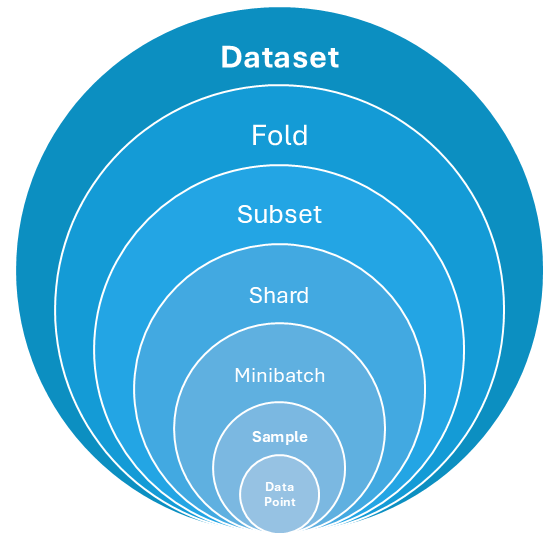
\includegraphics[width=0.4\columnwidth]{fig_datatier/DataTier-Onion.png} 
    \vspace{-0.2in}
    \caption{Depiction of data artifacts as containers of other data artifacts. \label{fig:datatier-onion}}
\end{figure}



The "onion" depiction of data artifacts encapsulates the hierarchical nature of data management within the MANOLO suite. At the core, there are data points, which aggregate into samples. These samples, can belong to mini-batches or shards of multiple mini-batches. The container for those are subsets for training, validation, and testing, which collectively constitute a fold of the dataset for k-Fold cross validation experiments. This layered approach covers any organization of data artifacts, emphasizing the generic approach and scalability of the data tier.

The MANOLO data tier supports a wide range of artifact types, addressing the diverse needs of modern applications. Object/Record Sets represent collections of objects or records with fields that can vary in data type, such as numeric, string, date, or nested objects. Vector Sets consist of fixed-dimensional numeric vectors with uniform data types and ranges, suitable for structured numerical data. Image Sets manage tensors representing grayscale, RGB, or RGB-D images. Point Cloud Sets handle spatial data in three dimensions, where samples are sets of points in a 3D coordinate system. Video Sets accommodate sequences of images over time, capturing dynamic visual data. Time-Series Sets store sensor recordings over time, representing scalar or vector values at discrete timestamps. Graph Datasets encode relationships through vertices and edges, represented in adjacency lists or matrices, with associated values. Spatiotemporal Graph Datasets extend this by incorporating temporal dimensions, allowing each vertex and each edge to have a time series of its values. 

\subsubsection{Experiment artifacts and model registries}
The MANOLO data tier extends its architecture to facilitate the hosting and management of machine learning experiments, encompassing models and associated artifacts. It offers the capability to seamlessly organize and connect various components of an ML experiment, beginning with the model itself and hyperparameters governing its architecture, the data handling and training processes. Each ML experiment is linked to a specific training set from a dataset, ensuring traceability and reproducibility of the training context. The data tier can store the final state of a trained model but also intermediate states during training, also known as checkpoints, including the model parameter state and the training process variable values. These artifacts enable pausing and resuming training sessions or evaluating different stages in a model's training process.

The relational structure of the MANOLO data tier ensures that all these components are interconnected. Models, training sets, and other associated artifacts are represented as objects with unique Object IDs (OIDs), while their relationships are captured using semantic triplets. This approach allows for defining the dependencies and associations between a model, its training data, and the parameters of its training process. Key-value pairs stored in metadata arrays further enrich these objects, providing additional context such as the provenance of the data, hyperparameter configurations, evaluation metrics, and any other relevant details.

The system accommodates various model-related artifacts, each with distinct roles. Model state objects (MS) represent the complete set of parameters and structural definitions for a pre-trained model, enabling efficient storage and retrieval of ready-to-use models. Training state objects (ST) capture the entire set of parameters necessary to resume a paused training session, which may include both the model and additional states related to the training algorithm. Model class objects (MC) define collections of related models, that are either generated during a hyperparameter search, or sharing common characteristics such as common architecture or dataset configurations. Finally, surrogate models (SM) are supported as explainable representations of non-explainable models, providing interpretability while maintaining the original model's predictive capabilities.

Through this architecture, the MANOLO data tier ensures that machine learning experiments are not only efficiently stored but also fully contextualized within a relational framework. By leveraging metadata, semantic relationships, and hierarchical object structures, the system supports complex ML workflows, enabling reproducibility, scalability, and adaptability without delving into the specific implementation details of individual methods.

\subsection{General purpose artifacts}
The data tier in MANOLO is designed to handle a wide variety of file types, accommodating diverse artifacts. These include plain text files such as unstructured text (.TXT) and tabular text formats (.CSV, .XLSX, .ODS), document files, and generic binary files like custom binary formats (.BIN) and compressed binary formats (.ZIP, .TAR). It also supports generic multimedia files, including original and compressed images, raw and encoded video formats. Additionally, the system manages raw and encoded signal data, as well as serialized objects in textual formats (.XML, .JSON) and binary serialized objects (e.g., Pickle, Protobuf). This generic approach allows MANOLO's data tier to handle both structured and unstructured data efficiently across various file types and formats.

\subsubsection{Metadata and semantic relations between artifacts}

Metadata can be attached to artifacts in a flexible way to support various project needs, such as recording metrics after evaluating experiments, or storing series of values from monitoring processes. Each object hosts an associative array to hold metadata in the form of key-value pairs, where the value may contain an objec with multiple fields (e.g., hyperparameter name-value pairs). Metadata can also be structured as a tree, allowing annotations to follow a hierarchical structure. Moreover, they can be organized in any kind of graph, utilizing an adjacency list or matrix for representing complex relationships.

Additionally, semantic triples in the form of subject-predicate-object, are used to define logical relations between artifacts, such as “dataset A is reduced into dataset B” or “model B is an alternative to model A,” providing semantic meaning to the connections between different entities. For tasks requiring relational data, the metadata can be structured as relational rows, where each row corresponds to a set of related values. This flexibility in metadata structure allows MANOLO to support a wide range of tasks, from data reduction and model comparison to more complex monitoring and evaluation processes.

Furthermore, the data tier in MANOLO supports basic querying on these semantic relations, enabling users to easily retrieve useful information to facilitate project tasks. For example, users can query to "list all alternatives of model A" or "list all derived datasets of dataset A," making it easier to explore the relationships between artifacts and enabling more efficient project management and decision-making.

\subsection{Manolo data tier web service}
The MANOLO data tier is a robust and scalable web service built using .NET Core, designed to efficiently handle and store various types of artifacts and metadata. It operates as a \textbf{FastAPI} web service, enabling seamless communication with other systems through standard HTTP methods (GET, POST, PUT, DELETE). This service is deployed within a Docker container, ensuring ease of deployment, scalability, and isolation. It can be deployed on the cloud for shared access or inside the local network edge for isolated use.


The core data management suite of the system is PostgreSQL, an SQL-compatible database that also supports NoSQL features through JSON and JSONB data types. PostgreSQL allows the creation of tables to store structured data, with each data structure (e.g., experiments, models, datasets) having its own dedicated table. For enhanced performance, PostgreSQL is configured with Generalized Inverted Indexes (GIN) to index JSON and JSONB columns, enabling fast and efficient querying of non-relational data. It also supports full-text search capabilities, crucial for querying metadata stored in JSON/JSONB format.
For file storage, MANOLO utilizes the standard Linux file system (ext4) within the Docker container. Files are organized according to the Linux directory structure, ensuring compatibility and ease of access. This system is well-suited for storing large artifacts such as models, datasets, and experiment logs.

Each artifact or metadata entry in MANOLO is associated with a unique identifier, typically a \textbf{Unique Lexicographically Sortable Identifier (ULID)} ensuring global uniqueness across distributed systems. These ULIDs are used to reference and access individual records across the data tier. The system handles a wide range of data types, including structured data (e.g., tabular data, hyperparameters) stored in PostgreSQL tables and unstructured or semi-structured data (e.g., JSON/JSONB, raw files) stored in both PostgreSQL and NoSQL databases. Object of large volume, like model states or large-scale datasets, can also be stored in an auxiliary tensor store database to leverage high-performance operations and efficient storage schemes.

In the MANOLO system, each artifact type has a specific table in the database. For every data structure entry, a corresponding table named Items is created within the PostgreSQL database. Each record in the table contains a unique identifier implemented using ULIDs, a data field capable of storing variable-sized content in byte format, a field that specifies the type of data stored, and a timestamp that tracks the last modification of the entry. This design provides a generic approach to storing any artifact within the MANOLO framework.

The MANOLO data tier employs robust security measures to safeguard the confidentiality, integrity, and proper access control of artifacts. User authentication is managed through cookie-based authentication, which is mandatory for accessing or interacting with system endpoints. Each endpoint is governed by a designated authorization policy, with access determined by the cookie issued to the user during the sign-in process. This mechanism allows for the definition of access attribute flags tailored to each endpoint's requirements.

The system currently supports three authentication policies:
\begin{itemize}
    \setlength{\itemsep}{0pt}
    \setlength{\parskip}{0pt}
    \item \textbf{All}, which grants access to endpoints open to all users;
    \item \textbf{ModeratorOrHigher}, which permits access to most endpoints; and
    \item \textbf{AdminOnly}, which provides access to all endpoints.
\end{itemize}

These access logs allow for detailed tracking and auditing of user activity, helping detect unauthorized access and ensure compliance with security policies.

For data protection, MANOLO supports both encryption during transfer and storage. Data in transit is protected using transport layer encryption, such as TLS 1.3, to ensure confidentiality and integrity while being transmitted. For storage encryption, artifact objects that are not actively queried or are infrequently accessed could be encrypted when stored using symmetric end-to-end encryption, such as AES-256. Importantly, the symmetric encryption uses the end user to manage their encryption key, ensuring they maintain full control over access to sensitive data. This encryption process ensures that only authorized users with the correct decryption keys can access sensitive artifact content. Overall, the combination of authentication, access control, access logging, and encryption provides a strong security framework to safeguard data throughout the lifecycle of the project.

\subsection{Data tier web API reference}
The Data Tier Web API Reference provides an overview of the key endpoints used for managing data within the system. It covers operations for creating, retrieving, updating, deleting and restoring various entities such as data structures, items, predicates, relations, aliases and key-value pairs. Additionally, it includes authentication and management functionalities, such as user login and database backup and restore. Each section outlines available endpoints, their purpose, and the parameters required, offering a clear and concise framework for interacting with the API. This reference is designed to help efficiently utilize the system’s capabilities while ensuring consistency and reliability in data management.


\subsubsection{Data Structures}
%=================================================================================================
\begin{longtable}
    \centering
    \renewcommand{\arraystretch}{1.2}
    \begin{tabular}{|p{0.25\linewidth}|p{0.75\linewidth}|}
% -----------------------------------------------------------------------
\hline
    \underline{Method Name} & \underline{Description} 
\\
% -----------------------------------------------------------------------    
\hline \textbf{GetDataStructures} & Summary: Handles the request to retrieve a list of data structures from the database.

Returns: A Result object containing a list of data structure IDs if any exist, or a failure result with a domain error if no data structures are found.
\\       
% ----------------------------------------------------------------------- 
\hline \textbf{CreateDataStructure} & Summary: Handles the creation of a new data structure.

Parameters:

- Request: The CreateDataStructureQuery containing the details of the data structure to be created.

Returns: A Task that represents the asynchronous operation. The task result contains a Result object. If successful, the Result contains the ID of the newly created data structure. If a data structure with the same name or DSN already exists, the Result indicates a failure with an appropriate error message.
\\     
% -----------------------------------------------------------------------
\hline \textbf{DeleteDataStructure} & Summary: Handles the deletion of a DataStructure based on the provided request.

Parameters:

- Request: The request containing the DataStructures ID, DSN, or Name to be deleted.

Returns: A Result object indicating the success or failure of the deletion operation, along with any relevant error messages.
\\
% -----------------------------------------------------------------------
\hline \textbf{GetDataStructure} & Summary: Summary: Handles the request to get a specific data structure by its ID.

Parameters:

- Request: The request containing the ID of the data structure to retrieve.

Returns: A Result object containing the retrieved data structure if it exists, or a failure result with a domain error if the data structure does not exist.
\\
% -----------------------------------------------------------------------
\hline \textbf{RestoreDataStructure} & Summary: Handles the request to restore a data structure.

Parameters:

- Request: The request containing the data structures ID, DSN, or name to be restored.

Returns: A Result object indicating the success or failure of the restore operation, along with a message.
\\
% -----------------------------------------------------------------------
\hline \textbf{UpdateDataStructure} & Summary: Handles the update of a data structure.

Parameters:

- Request: The request containing the data structures id and updated properties.

Returns: A Result object indicating the success or failure of the operation, along with any relevant error messages.
\\
% ----------------------------------------------------------------------- 

        \hline
    \end{tabular}
\end{longtable}
%=================================================================================================





\newpage
\subsubsection{Items}
%=================================================================================================
\begin{longtable}
    \centering
    \renewcommand{\arraystretch}{1.2}
    \begin{tabular}{|p{0.25\linewidth}|p{0.75\linewidth}|}
% -----------------------------------------------------------------------     
\hline
    \underline{Method Name} & \underline{Description} 
\\
% ----------------------------------------------------------------------- 
\hline
    \textbf{CreateItem} & Summary: Handles the creation of a new item based on the provided request.
    
Parameters:

- Request: The create item query containing the necessary data for item creation.

Returns: A task that represents the asynchronous operation. The result of the task is a Result object indicating success or failure, along with the new items ID.
\\
% ----------------------------------------------------------------------- 
\hline
    \textbf{DeleteItem} & Summary: Handles the deletion of an item based on the provided request.
    
Parameters:

- Request: The delete item query containing the DSN and item ID.

Returns: A Result indicating the success or failure of the deletion operation.
\\
% ----------------------------------------------------------------------- 
\hline
    \textbf{DownloadItemData} & Summary: Handles the download of item data based on the provided DSN and item ID.
    
Parameters:

- Request: The download item data query containing the DSN and item ID.

Returns: An IActionResult representing the downloaded file or a NotFoundResult if the item or data structures are not found.
\\
% ----------------------------------------------------------------------- 
\hline
    \textbf{GetItem} & Summary: Handles the GetItemQuery request by retrieving an item from the database based on the provided DSN and item ID.
    
Parameters:

- Request: The GetItemQuery request containing the DSN and item ID.

Returns: A Result object containing the retrieved item if successful, or an error message if the item does not exist or an error occurs.
\\
% ----------------------------------------------------------------------- 
\hline
    \textbf{GetItemData} & Summary: Handles the GetItemDataQuery request to retrieve item data based on the provided DSN and item ID.
    
Parameters:

- Request: The GetItemDataQuery request containing the DSN and item ID.

Returns: A Result object indicating the success or failure of the operation. If successful, the Result contains the decoded item data as a string. If unsuccessful, the Result contains a DomainError indicating the specific error.
\\
% ----------------------------------------------------------------------- 
\hline
    \textbf{GetItems} & Summary: Handles the GetItemsQuery request to retrieve a list of items based on the provided DSN.
    
Parameters:

- Request: The GetItemsQuery request containing the DSN.

Returns: A Result object indicating the success or failure of the operation. If successful, the Result contains a list of item IDs. If unsuccessful, the Result contains a DomainError indicating the reason for the failure.
\\
% ----------------------------------------------------------------------- 
\hline
    \textbf{RestoreItem} & Summary: Handles the restore operation for a specific item in the database.
    
Parameters:

- Request: The restore item query containing the DSN and item ID.

Returns: A Result indicating the success or failure of the restore operation.
\\
% ----------------------------------------------------------------------- 
\hline
    \textbf{UpdateItem} & Summary: Handles the update of an item in the database.

Parameters:

- Request: The update item query containing the necessary parameters.

Returns: A Result indicating the success or failure of the operation.
\\
% ----------------------------------------------------------------------- 
        \hline
    \end{tabular}
\end{longtable}
       
%=================================================================================================


\newpage
\subsubsection{Predicates}
%=================================================================================================
\begin{longtable}
    \centering
    \renewcommand{\arraystretch}{1.2}
    \begin{tabular}{|p{0.25\linewidth}|p{0.75\linewidth}|}
% -----------------------------------------------------------------------    
\hline
    \underline{Method Name} & \underline{Description} 
\\
% -----------------------------------------------------------------------
\hline
    \textbf{CreatePredicate} & Summary: Handles the creation of a new predicate.
    
Parameters:

- Request: The request containing the description of the predicate to be created.

Returns: A Result representing the asynchronous operation. The task result contains the unique identifier of the newly created predicate if successful, or an error message if the predicate already exists.
\\
% -----------------------------------------------------------------------
\hline
    \textbf{DeletePredicate} & Summary: Handles the deletion of a predicate based on the provided description.
    
Parameters:

- Request: The delete predicate query contains the description of the predicate to be deleted.

Returns: A task that represents the asynchronous operation. 	The task result is a Result indicating the success or failure of the operation. If the predicate with the given description does not exist, the result will be a failure with a corresponding error.
\\
% -----------------------------------------------------------------------
\hline
    \textbf{GetObjectsOfPredicate} & Summary: Handles the request to get objects related to a specific predicate.
    
Parameters:
- Request: The request containing the predicate description.

Returns: A Result object indicating success or failure. If successful, the Result contains a list of objects related to the predicate. If unsuccessful, the Result contains a DomainError indicating the reason for failure.
\\
% -----------------------------------------------------------------------
\hline
    \textbf{GetPredicates} & Summary: Handles the GetPredicatesQuery request to retrieve a list of predicates from the database.
   
Parameters:

- Request: The GetPredicatesQuery request object containing any necessary parameters.

Returns: A Result object indicating the success or failure of the operation. If successful, the Result contains a list of existing predicates. If unsuccessful, the Result contains a DomainError indicating the reason for the failure.
\\
% ----------------------------------------------------------------------- 
\hline
    \textbf{GetSubjectsOfPredicate} & Summary: Handles the request to retrieve subjects related to a specific predicate.
    
Parameters:

- Request: The request containing the predicate description.

Returns: A Result representing the asynchronous operation. The result contains either a list of subjects related to the predicate or an error message.
\\
% ----------------------------------------------------------------------- 
\hline
    \textbf{GetSubjectsOf} & Summary: Handles the GetSubjectsOfQuery request to retrieve the subjects related to a specific object.
    
Parameters:

- Request: The GetSubjectsOfQuery request containing the object and predicate description.

Returns: A Result object indicating the success or failure of the operation. 	If successful, the Result contains a list of related subjects. If unsuccessful, the Result contains a DomainError indicating the reason for the failure.
\\
% ----------------------------------------------------------------------- 
\hline
    \textbf{GetObjectsOf} & Summary: Handles the GetObjectsOfQuery request to retrieve objects related to a given subject.
    
Parameters:

- Request: The GetObjectsOfQuery request containing the subject and description.

Returns: A Result object indicating success or failure. If successful, the Result contains a list of related objects. If failure, the Result contains a DomainError indicating the reason for the failure.
\\
% ----------------------------------------------------------------------- 
        \hline
    \end{tabular}
\end{longtable}        
%=================================================================================================


\newpage
\subsubsection{Relations}
%=================================================================================================
\begin{longtable}
    \centering
    \renewcommand{\arraystretch}{1.2}
    \begin{tabular}{|p{0.25\linewidth}|p{0.75\linewidth}|}
% -----------------------------------------------------------------------     
\hline
    \underline{Method Name} & \underline{Description} 
\\
% ----------------------------------------------------------------------- 
\hline
    \textbf{CreateRelation} & Summary: Handles the creation of a new relation between two entities (subject and object) based on the given predicate and 	DSN.
    
Parameters:

- Request: The create relation query containing the necessary parameters.

Returns: A task that represents the asynchronous operation. 	The result is an indication of success or failure. If successful, the result is Result.Success; otherwise, it is Result.Failure with an appropriate error.
\\
% ----------------------------------------------------------------------- 
\hline
    \textbf{DeleteRelation} & Summary: Handles the deletion of a relation between two entities in the ManoloDataTier system.
    
Parameters:

- Request: The delete relation query containing the details of the relation to be deleted.

Returns: A Result indicating the success or failure of the deletion operation.
\\
% ----------------------------------------------------------------------- 
\hline
    \textbf{GetRelations} & Summary: Handles the GetRelationsQuery request to retrieve a list of relations from the database.
    
Parameters:

- Request: The GetRelationsQuery request containing any necessary parameters.

Returns: A Result object containing either a list of relations or an error message. If the list of relations is empty, it returns a failure Result with a NoRelations domain error. Otherwise, it returns a success Result with the list of relations.
\\
% ----------------------------------------------------------------------- 
\hline
    \textbf{AddChild} & Adds a child item object under a parent item object in a tree data structure.
    
Parameters:

- DSN: data structure number.

- Parent: parent object ID

- Child: child object ID
\\
% ----------------------------------------------------------------------- 
\hline
    \textbf{GetChildren} & Return a list with the object IDs for the children of the given parent item in a tree data structure.
    
Parameters:

- DSN: data structure number.

- Parent: parent object ID
\\
% ----------------------------------------------------------------------- 
\hline
    \textbf{AddEdge} & Add an edge between two node item objects in a graph data structure.
    
Parameters:

- DSN: data structure number.

- node1:  first (source) node object ID

- node2:  second (destination) node object ID

- value (optional):  the value for the edge

- is\textunderscore directed (optional): | 0 (default) undirected edge | 1: directed edge. 
\\
% ----------------------------------------------------------------------- 
\hline
    \textbf{GetAdjacencyList} & Return a list with the object IDs for the adjacent nodes to the given node item in a graph data structure.
    
Parameters:

- DSN: data structure number.

- node: node object ID.
\\
% ----------------------------------------------------------------------- 
        \hline
    \end{tabular}
\end{longtable}       
%=================================================================================================



\newpage
\subsubsection{Global Aliases}
%=================================================================================================
\begin{longtable}{c}
    \renewcommand{\arraystretch}{1.2}
    \begin{tabular}{|p{0.25\linewidth}|p{0.75\linewidth}|}
% -----------------------------------------------------------------------     
\hline
    \underline{Method Name} & \underline{Description} 
\\
% ----------------------------------------------------------------------- 
\hline
    \textbf{CreateUpdateAlias} & Summary: Handles the creation or update of an alias.
    
Parameters:

- Request: The CreateUpdateAliasQuery containing the alias details to be created or updated.

Returns: A Task that represents the asynchronous operation, containing a Result object. The Result is successful if the alias was created or updated, or a failure if an alias with the same name already exists.
\\
% ----------------------------------------------------------------------- 
\hline
    \textbf{DeleteAlias} & Summary: Handles the deletion of an alias based on the provided query.
    
Parameters:

- Request: The DeleteAliasQuery containing the alias name to be deleted.

Returns: A Result object indicating the outcome of the deletion operation. It would be a Success result if the alias was successfully deleted, or a Failure result with an AliasDoesNotExist error if no alias was found.
\\
% ----------------------------------------------------------------------- 
\hline
    \textbf{GetAlias} & Summary: Handles the GetAliasQuery request by retrieving an alias from the database.

Parameters:

- Request: The GetAliasQuery containing the ID of the alias to retrieve.

Returns: A Result object containing: 	

- Success with the alias name if the alias is found. 	

- Failure with a DomainError if the alias is not found.
\\
% ----------------------------------------------------------------------- 
\hline
    \textbf{GetId} & Summary: Handles the GetIdQuery request by retrieving the ID of an alias from the database.
    
Parameters:

- Request: The GetIdQuery object containing the alias name to search for.

Returns: A Result object containing either: 	- A successful result with the ID of the found alias, or 	- A failure results in an AliasDoesNotExist error if the alias is not found.
\\
% ----------------------------------------------------------------------- 
        \hline
    \end{tabular}
\end{longtable}      
%=================================================================================================



\newpage
\subsubsection{Key-Value Pairs}
%=================================================================================================
\begin{longtable}{c}
    \renewcommand{\arraystretch}{1.2}
    \begin{tabular}{|p{0.25\linewidth}|p{0.75\linewidth}|}
% -----------------------------------------------------------------------     
\hline
    \underline{Method Name} & \underline{Description} 
\\
% ----------------------------------------------------------------------- 
\hline
    \textbf{CreateUpdateKeyValue} & Summary: Handles the creation or update of a Key-Value pair in the database.

Parameters:

- Request: The request containing the Key-Value data.

Returns: A Result indicating the success or failure of the operation.
\\
% ----------------------------------------------------------------------- 
\hline
    \textbf{DeleteKeyValue} & Summary: Handles the deletion of a key-value pair from the database.
    
Parameters:

- Request: The delete key-value query containing the key to be deleted.

Returns: A Result representing the asynchronous operation. The result is an indication of success or failure. If the key does not exist in the database, the result will be a failure with a corresponding error.
\\
% ----------------------------------------------------------------------- 
\hline
    \textbf{GetKeys} & Summary: Handles the GetKeysQuery request to retrieve all keys associated with a specific object.
    
Parameters:

- Request: The GetKeysQuery request containing the object for which keys are requested.

Returns: A Result object indicating the success or failure of the operation. If successful, the Result contains a list of keys associated with the object. If unsuccessful, the Result contains a DomainError indicating the reason for the failure.
\\
% ----------------------------------------------------------------------- 
\hline
    \textbf{GetValue} & Summary: Handles the logic for retrieving a value associated with a given key from the database.
    
Parameters:

- Request: The request containing the key to retrieve.

Returns: A Result representing the asynchronous operation. The result is a Result object containing the retrieved value if the key exists, or an error message if the key does not exist.
\\
% ----------------------------------------------------------------------- 
        \hline
    \end{tabular}
\end{longtable}     
%=================================================================================================



\subsubsection{Authentication}
%=================================================================================================
\begin{longtable}{c}
    \renewcommand{\arraystretch}{1.2}
    \begin{tabular}{|p{0.25\linewidth}|p{0.75\linewidth}|}
% -----------------------------------------------------------------------     
\hline
    \underline{Method Name} & \underline{Description} 
\\
% ----------------------------------------------------------------------- 
\hline
    \textbf{AddUser} & Summary: Handles the addition of a new user to the database.
    
Parameters:

- Request: The AddUserQuery containing the new user's information.

Returns: A Task that represents the asynchronous operation, containing a Result object. The Result is successful if the user was added, or a failure with an error message if the username already exists.
\\
% ----------------------------------------------------------------------- 
\hline
    \textbf{Login} & Summary: Handles the login process for a user.
    
Parameters:

- Request: The login query containing the username and password.

Returns: A Result object indicating the outcome of the login attempt. Returns a success result if the login is successful, or a failure result if the user does not exist or the password is  incorrect.
\\
% ----------------------------------------------------------------------- 
\hline
    \textbf{Logout} & Summary: Handles the logout process for the current user.
    
Returns: A Result object indicating the success of the logout operation.
\\
% ----------------------------------------------------------------------- 
        \hline
    \end{tabular}
\end{longtable}       
%=================================================================================================



\newpage
\subsubsection{Management}
%=================================================================================================
\begin{longtable}{c}
    \renewcommand{\arraystretch}{1.2}
    \begin{tabular}{|p{0.25\linewidth}|p{0.75\linewidth}|}
% -----------------------------------------------------------------------     
\hline
    \underline{Method Name} & \underline{Description} 
\\
% ----------------------------------------------------------------------- 
\hline
    \textbf{Backup} & Summary: Handles the backup request by retrieving data from the database and storing it in a JSON file.
    
Returns: A Result indicating the success or failure of the backup operation.
\\
% ----------------------------------------------------------------------- 
\hline
    \textbf{Restore} & Summary: Handles the restore operation by processing the backup data and restoring it to the database.
    
Parameters:

- Request: The restore query containing the backup data.

Returns: A task that represents the asynchronous operation. The result is an indication of success or failure.
\\
% ----------------------------------------------------------------------- 
        \hline
    \end{tabular}
\end{longtable}    
%=================================================================================================

\clearpage
\section{Data Quality Estimation}
\label{sec:datqual}
% (M5-M24) Leader: NCSR "D"
% CeADAR, UPC, ATOS, EVIDEN, FDI, INRIA, ARCADA, use case partners

\subsection{Introduction}

In this research, we aim to develop a task-agnostic framework for time-series data quality estimation. Towards this goal, we propose methods for anomaly and noise detection, which allow us to identify biased, noisy, inconsistent, or otherwise low-quality data, as well as data that may have been maliciously manipulated to contaminate the model during training.

As a case study to validate our methods, we use the Bitbrain dataset, which consists of EEG signals collected from a headband across 128 recordings. This headband includes two EEG channels synchronized with medical-grade EEG devices. The signals are annotated by three experts, with each 30-second segment classified into one of five sleep stages: Wake, N1, N2, N3, and REM. These stages correspond to specific brain activity patterns, such as slow eye movements, sleep spindles, and other characteristic waveforms.

To further validate the robustness of our proposed methods, we explore data augmentation techniques, including adversarial machine learning methods that introduce controlled noise contamination into the dataset.

\subsection{Problem Statement}

The quality of time-series data plays a crucial role in the performance of machine learning models, yet existing methods often fail to effectively identify and handle noise in a task-agnostic manner. Traditional data quality estimation techniques are typically tailored to specific datasets, limiting their applicability to a wider range of applications. 

In this research, we address this limitation by developing a flexible framework that estimates data quality, with respect to noise, anomalies, and malicious manipulation, across different time-series datasets, regardless of the specific task or domain. This approach is commonly referred to as task-agnostic data quality estimation.

\subsection{Proposed Methodology}

We propose a task-agnostic framework for time-series data quality estimation, using a combination of machine learning-based and statistical approaches to detect noise and anomalies in data. The primary techniques used in this framework include:

\begin{enumerate}
    \item[(a)] Unsupervised machine learning with autoencoders, which compress the data and detect noise based on reconstruction errors.\\
    \vspace{-0.8cm}
    \item[(b)] Supervised machine learning with a transformer model, which uses attention mechanisms to identify noisy segments in the data.\\
    \vspace{-0.8cm}
    \item[(c)] Statistical approaches which detect noise based on changes in data characteristics over time.
\end{enumerate}

To apply these techniques, we implement the following 8 methods: LSTM Autoencoder, Convolutional LSTM Autoencoder, Attention-based Autoencoder, Transformer, MNE Filtering, Cumulative Sum Control, Page-Hinkley Test and Kullback-Leibler Divergence. The last 3 statistical methods are implemented using the \href{https://github.com/IFCA-Advanced-Computing/frouros}{Frouros} framework.

In our analysis, we chose to estimate noise across 30-second segments of the EEG data, which, in the Bitbrain dataset, corresponds to 7,680 samples. Since each method outputs noise values in different scales, we transform these values into binary based on predefined thresholds per channel to establish a common ground for comparison.

\subsection{Machine Learning Approach}
The general concept of using machine learning (ML) for noise estimation revolves around training models to solve specific tasks and then using their outputs during inference to estimate noise. These tasks may vary in nature — ranging from signal reconstruction and prediction to classification — but the core idea is that the model’s performance on these tasks can be used to infer the presence of noise.

To train the models, we split the dataset into training (43 recordings), validation (3 recordings), and testing subsets (10 recordings). Noise estimation is performed using the test dataset. For the training configuration, we set the batch size to 512 and train the models for a maximum of 1000 epochs. To prevent overfitting, we employ early stopping with a patience of 30 epochs, meaning that if the validation loss does not improve for 30 consecutive epochs, training will stop. We set the learning rate to $1e^{-4}$ and use the Adam optimizer to adjust the model weights. Additionally, we implement a \emph{ReduceLROnPlateau} scheduler to dynamically adjust the learning rate based on the validation loss. If the validation loss plateaus, the scheduler reduces the learning rate to help the model continue improving.

To ensure robust model training and reliable outcomes, we rely on data preprocessing techniques. Proper preprocessing standardizes the input data, mitigates inconsistencies, and enhances the model’s ability to learn meaningful representations. In our case, preprocessing involves handling missing or ambiguous data by removing rows containing NaN values, as well as any samples where expert annotators could not agree on the class label (i.e., samples with a label value of 8). Additionally, we apply normalization to assist model training by making the data more uniform. Due to the low variability and the presence of extreme outliers in the EEG signals, we adopt a robust normalization approach. Instead of using the mean and standard deviation, which are sensitive to outliers, we use the median and interquartile range (IQR). We scale the data based on statistics computed across the entire dataset, rather than on a per-batch basis, since the statistics remain consistent across the full dataset.

\begin{equation}
    x_{\text{norm}} = \frac{x - \text{median}(x)}{\text{IQR}(x)} \label{eq:robust_norm}
\end{equation}

where $x$ represents the values of a particular feature, $\text{median}(x)$ is the median value of the feature, and $\text{IQR}(x)$ is the interquartile range, which measures the spread of the middle 50\% of the data. We use the median as a measure of central tendency because it is robust against extreme values, making it a more reliable indicator for our dataset, which exhibits low variability and where even small differences matter. Additionally, we use the interquartile range $\text{IQR} = Q_3 - Q_1$ to reduce the influence of outliers by focusing on the range within which the central portion of the data lies. This approach ensures that our normalization process allows the model to learn from the true patterns in the dataset.

For all machine learning methods, we need to establish a common standard to determine what is considered noise and what is not. As the models output different value ranges, we need a policy to classify these outputs into binary values that indicate noise presence or absence. One such approach involves defining thresholds that act as a boundary between noise and clean data. For these methods, we define thresholds based on the 75th percentile of noise values for each channel. Values above the thresholds are set to 1 (indicating noise), while those below are set to 0 (indicating no noise).

Noise estimation within this machine learning approach can be divided into two categories: label-based and label-free:

\begin{itemize}
    \item The label-based approach involves training classifier models on labeled data to learn how to assign class labels to signals. The \emph{Transformer Classifier}, trained to classify signals into sleep stages, belongs to this category. The idea is to use the model’s attention matrix, which highlights the importance of different time steps in data, to infer the presence of noise. Higher attention values correspond to segments of data that are likely noisy, whereas lower attention values indicate cleaner segments of data.
    \vspace{-0.2cm}
    \item The label-free approach does not rely on labeled data for training. Instead, it focuses on unsupervised or semi-supervised techniques to estimate noise based on the characteristics of the signal itself. In this category, we use models like autoencoders and transformers that learn to reconstruct or predict signals. The 3 \emph{Autoencoders} as well as the \emph{Transformer Predictor} are examples of models used in this approach. These models are trained to reconstruct the input data, and noise is mainly identified through the reconstruction error — the larger the error, the more likely the segment is noisy. Additionally, the attention-based models, \emph{Attention-based Autoencoder} and \emph{Transformer Predictor}, can also estimate noise using the attention matrix. Just like in the label-based approach, higher attention values indicate segments of data that are likely noisy, while lower attention values correspond to cleaner segments.
\end{itemize}

\subsubsection{LSTM Autoencoder}

We implement an LSTM-based autoencoder to transform EEG signals into a lower-dimensional latent representation. The key idea behind this approach is to compress the input signal while preserving the essential features, then reconstruct it from the compressed representation. The LSTM layers in the encoder are designed to capture the temporal patterns and dependencies inherent in the EEG signals. These temporal dependencies are crucial for accurately modeling EEG data, which often exhibits long-range correlations over time. The decoder, in turn, reconstructs the original signal from this latent representation, hoping that only non-noisy information is preserved during compression.

To process the input data, we split each 30-second segment of EEG data into 32 smaller chunks, resulting in 240 sequences per segment. Each sequence has a length of 240 time steps, with 2 features corresponding to the EEG channels. This structure allows the model to focus on both the short- and long-term temporal dependencies within the data. The encoder processes each sequence and compresses it into a latent representation of size (1, 8), where the first dimension represents a single compressed time step, and the second dimension represents 8 learned features. The decoder then takes this compressed representation and attempts to reconstruct the original signal, capturing both trends and amplitudes.

To balance the models' focus on both the amplitude and trends of the EEG signals, we define a custom loss function, called \emph{BlendedLoss}. This function combines the median and mean of the powered absolute differences between the predicted ($\hat{x}$) and target values ($x$):
%
\begin{equation}
\text{Loss} = (1 - \text{blend}) \cdot \text{median}(\lvert \hat{x} - x \rvert^p) + \text{blend} \cdot \text{mean}(\lvert \hat{x} - x \rvert^p)
\label{eq:blended_loss}
\end{equation}
%
where $p$ is the power parameter that controls the sensitivity of the loss to the differences, $x$ is the original signal, and $\hat{x}$ is the reconstructed signal. The blend factor controls the trade-off between learning the overall trends (via the median) and capturing the amplitude (via the mean). We experiment with different blend values (0.1 and 0.8) to observe how this affects the model’s performance in reconstructing the signals.

The LSTM Autoencoder estimates noise by measuring the reconstruction error between the original and the reconstructed signal. During training, the model learns to compress and then reconstruct the input signal with minimal error. The goal is for the model to capture the common patterns and trends in the data, such as periodic fluctuations or typical signal behavior. When the model encounters unusual spikes, often caused by noise, it struggles to reconstruct them because they don't fit the typical patterns it has learned. As a result, the reconstruction error for these segments will be larger, indicating noise.

\subsubsection{Convolutional LSTM Autoencoder}

We implement a ConvLSTM-based autoencoder to transform EEG signals into a lower-dimensional latent representation, combining the strengths of both convolutional and LSTM layers. The convolutional layers help capture local features in the data, while the LSTM layers capture the long-range temporal dependencies. This hybrid approach is particularly effective for spatiotemporal data like EEG signals, where both spatial (local) and temporal (long-range) patterns are important.

The data processing approach (splitting EEG segments into 32 smaller chunks) remains the same as in the LSTM-based autoencoder. We use the same \emph{BlendedLoss} function, as defined in Equation~\ref{eq
}, to balance the reconstruction of amplitude and trends. Similar to the LSTM approach, noise is estimated through the reconstruction error.

\subsubsection{Attention-based Autoencoder}
...
The \emph{BlendedLoss} function as defined in Equation~\ref{eq:blended_loss}, is also used for the attention-based autoencoder, ensuring consistency across all autoencoders.

\subsubsection{Transformer Predictor}
....

\subsubsection{Transformer Classifier}
....
%Classifies sleep stages using attention mechanisms. Noise is identified in parts of the signal that get lower attention scores during inference. These are less informative for feature-label associations, likely due to the disruptive effect of noise.
...
To train the model, we use Cross-Entropy loss, which measures the dissimilarity between the predicted probability distribution and the true distribution. This loss function is commonly used for classification problems to penalize the model based on how confident and accurate its predictions are. Given that the dataset is quite imbalanced, with class frequencies reflected by the weights as shown in Table \ref{tab:class_freqs_weights}, we employ a weighted version of the Cross-Entropy loss (see: Equation~\ref{eq:weighted_cross_entropy_loss}). This approach adjusts the influence of each class in the loss calculation, helping the model learn across all class distributions, regardless of their prevalence in the dataset.

\begin{equation}
    \text{Loss} = -\sum_{i=1}^{N} w_{y_i} \cdot \log(p_{y_i})
    \label{eq:weighted_cross_entropy_loss}
\end{equation}

where \(N\) is the total number of samples, \(y_i\) represents the true class label for the \(i\)-th sample, \(p_{y_i}\) is the predicted probability for the true class, and \(w_{y_i}\) is the weight assigned to the class \(y_i\).

\begin{table}[h!]
    \centering
    \begin{tabular}{c|c|c}
    Class & Freqs (\%) & Weights \\
    \hline
    0 & 14.11 & 0.12 \\
    1 & 4.45  & 0.39 \\
    2 & 62.16 & 0.03 \\
    3 & 4.96  & 0.35 \\
    4 & 14.36 & 0.12 \\
    \end{tabular}
    \caption{Class frequencies and weights used in weighted cross-entropy loss.}
    \label{tab:class_freqs_weights}
\end{table}

\subsection{Statistical Approach}
....
Preprocessing for the statistical methods is similar to that of the machine learning-based methods in terms of handling NaN values and ambiguous samples. However, unlike the machine learning methods, no normalization is applied, as the statistical methods require the raw data to function.
....
For MNE filtering, the noise thresholding approach is consistent with the machine learning-based methods, using the 75th percentile to separate noise (1) from no noise (0). On the other hand, the Frouros-based methods inherently provide binary outputs. To handle cases where sample aggregation results in float values, we apply a threshold of 0.5 to convert these results into binary form.
...
To ensure consistency across all methods and enable meaningful comparisons, the same test recordings used for machine learning-based noise estimation are also applied to the statistical methods.
... 

\subsubsection{MNE Filtering}
...
%Applies bandpass filtering to the input signals to remove noise outside a specified frequency range (0.5 to 40 Hz). Noise is estimated as the difference between the original and the filtered version.
....

\subsubsection{Cumulative Sum Control}
...

\subsubsection{Page-Hinkley Test}
...

\subsubsection{Kullback-Leibler Divergence}
...








\subsubsection{Cumulative Sum Control}
Tracks the cumulative sum of deviations from a target mean over time. Noise is detected when the cumulative sum of these deviations exceeds a threshold.

\subsubsection{Page-Hinkley Test}
Compares the cumulative mean of observed values to the global mean of the data. Noise is detected when the cumulative mean diverges from the global mean beyond a threshold.

\subsubsection{Kullback-Leibler Divergence}
Measures the difference between probability distributions of two consecutive data windows. Noise is estimated when the divergence exceeds a threshold.






%%%%%%%%%%%%%%%%%%%%%%%%%%%%%%%%%%%%%%%%%%%%%%%%%%%%%%%%%%%%%%%%%%%%%%%%%%%%%%%%%%%%%%%%%%%%%%%%%%%%%%%%%%%%%%%
% During the experiments, we focus on evaluating how well the decoder reconstructs the latent representations back into their original form. We compare the original signal with the decoded version, not only visually through plots but also by using various metrics to quantify performance. Since the testing data is quite large, we select one random batch for analysis. This batch is visualized using two subplots, one for each EEG feature, representing the signal for each channel separately.

% \subsection{Signal Comparison} First, we plot the original and decoded signals, where the x-axis represents the samples and the y-axis shows the amplitude of the signal.

% When the blend is set to 0.1, the decoded signal effectively captures the tendencies and patterns of the original signal, though its amplitude is significantly restricted, centering around zero. The original signal displays larger amplitudes, with values ranging from approximately 3 to -9.
% %
% \begin{figure}[ht]
%     \centering
%     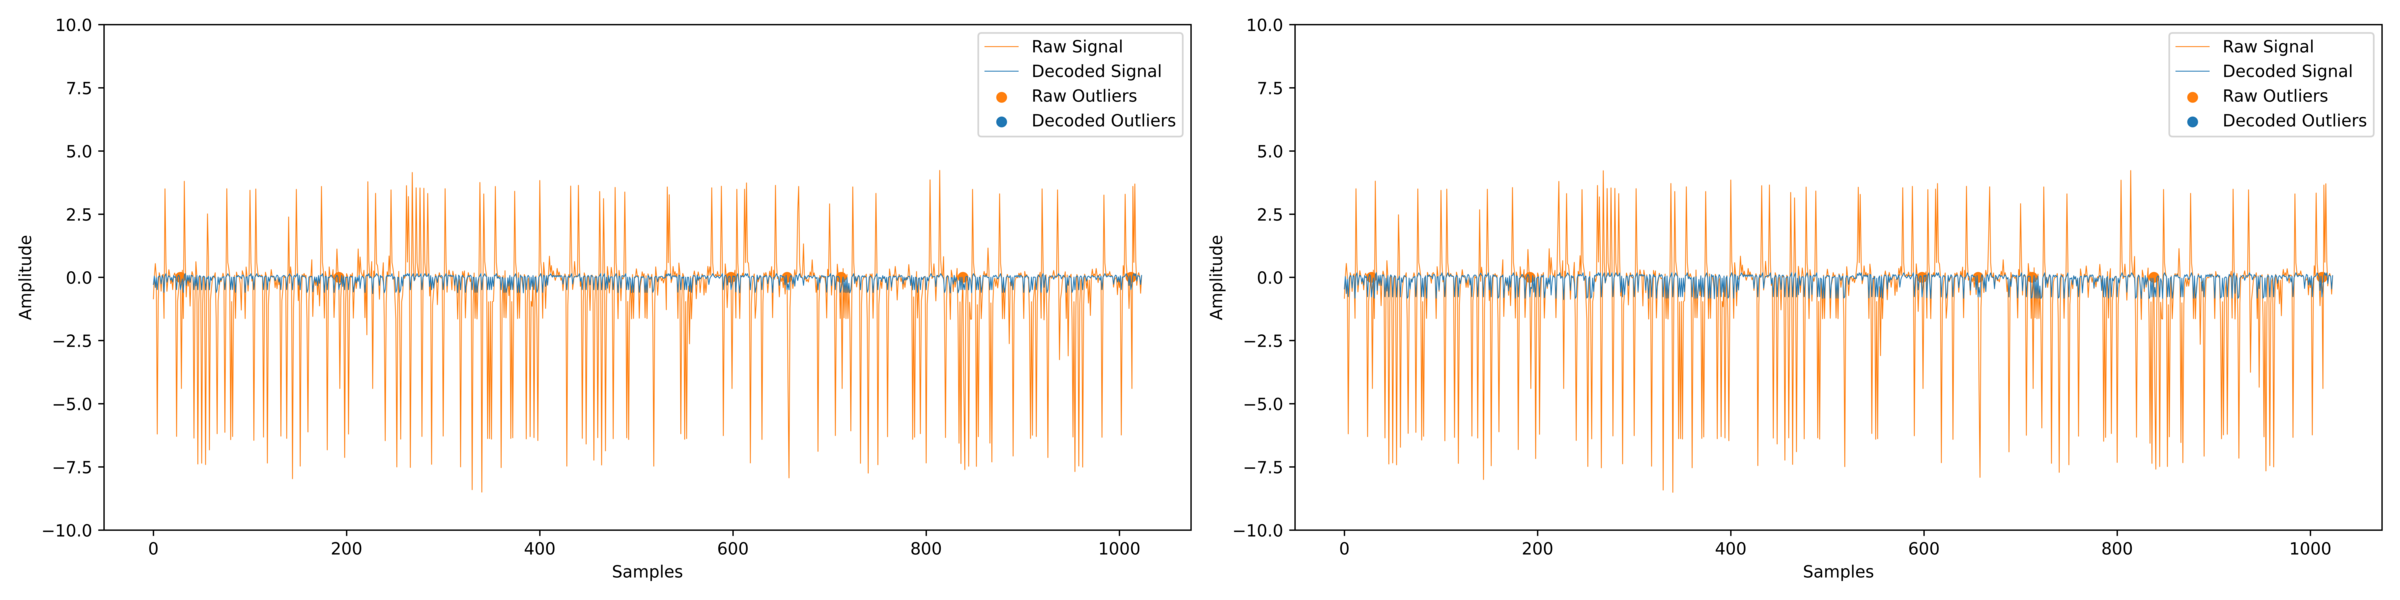
\includegraphics[width=0.8\textwidth]{static/original_vs_decoded_blend_01_resized.png}
%     \caption{Signals when blend=0.1}
%     \label{fig:signal_01}
% \end{figure}
% %
% When the blend is set to 0.8, the decoded signal captures the patterns and flow of the original signal more accurately, with amplitudes reaching up to approximately $\pm0.5$. This improvement demonstrates that increasing the focus on the mean in the loss function results in an overall better reconstruction of the original signal.
% %
% \begin{figure}[ht]
%     \centering
%     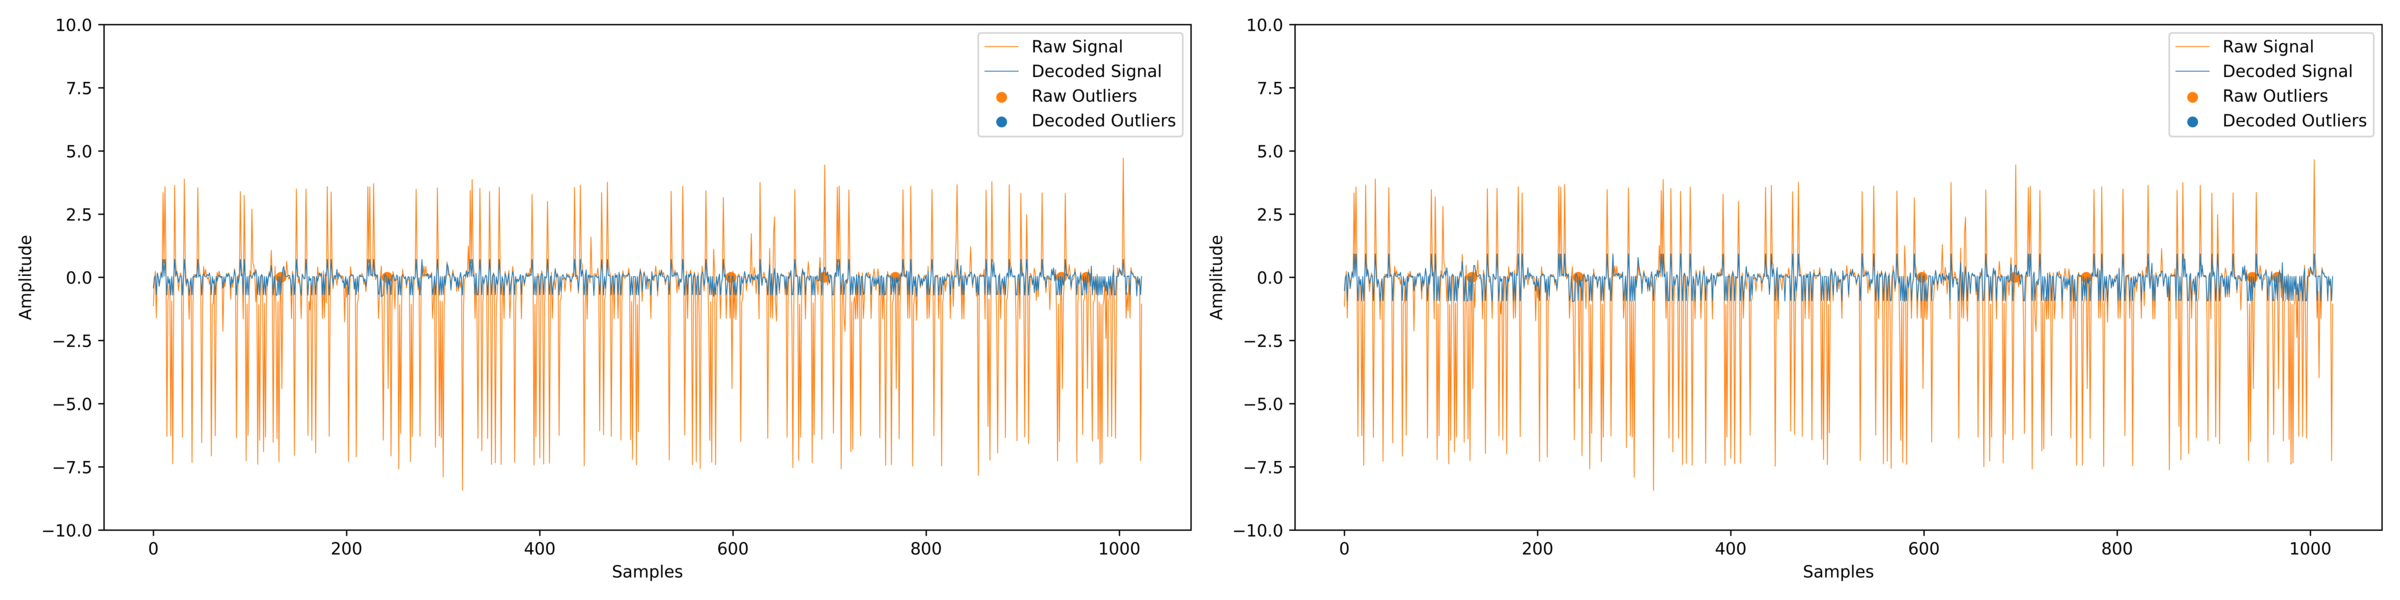
\includegraphics[width=0.8\textwidth]{static/original_vs_decoded_blend_08_resized.png}
%     \caption{Signals when blend=0.8}
%     \label{fig:signal_08}
% \end{figure}
% %

% \subsubsection{Detrended Signal Comparison} We also analyze the detrended signal using the Theil-Sen estimator. For both the 0.1 and 0.8 blends, the detrended signal trends are nearly flat, indicating minimal differences between the original and decoded signals.
% %
% \begin{figure}[ht]
%     \centering
%     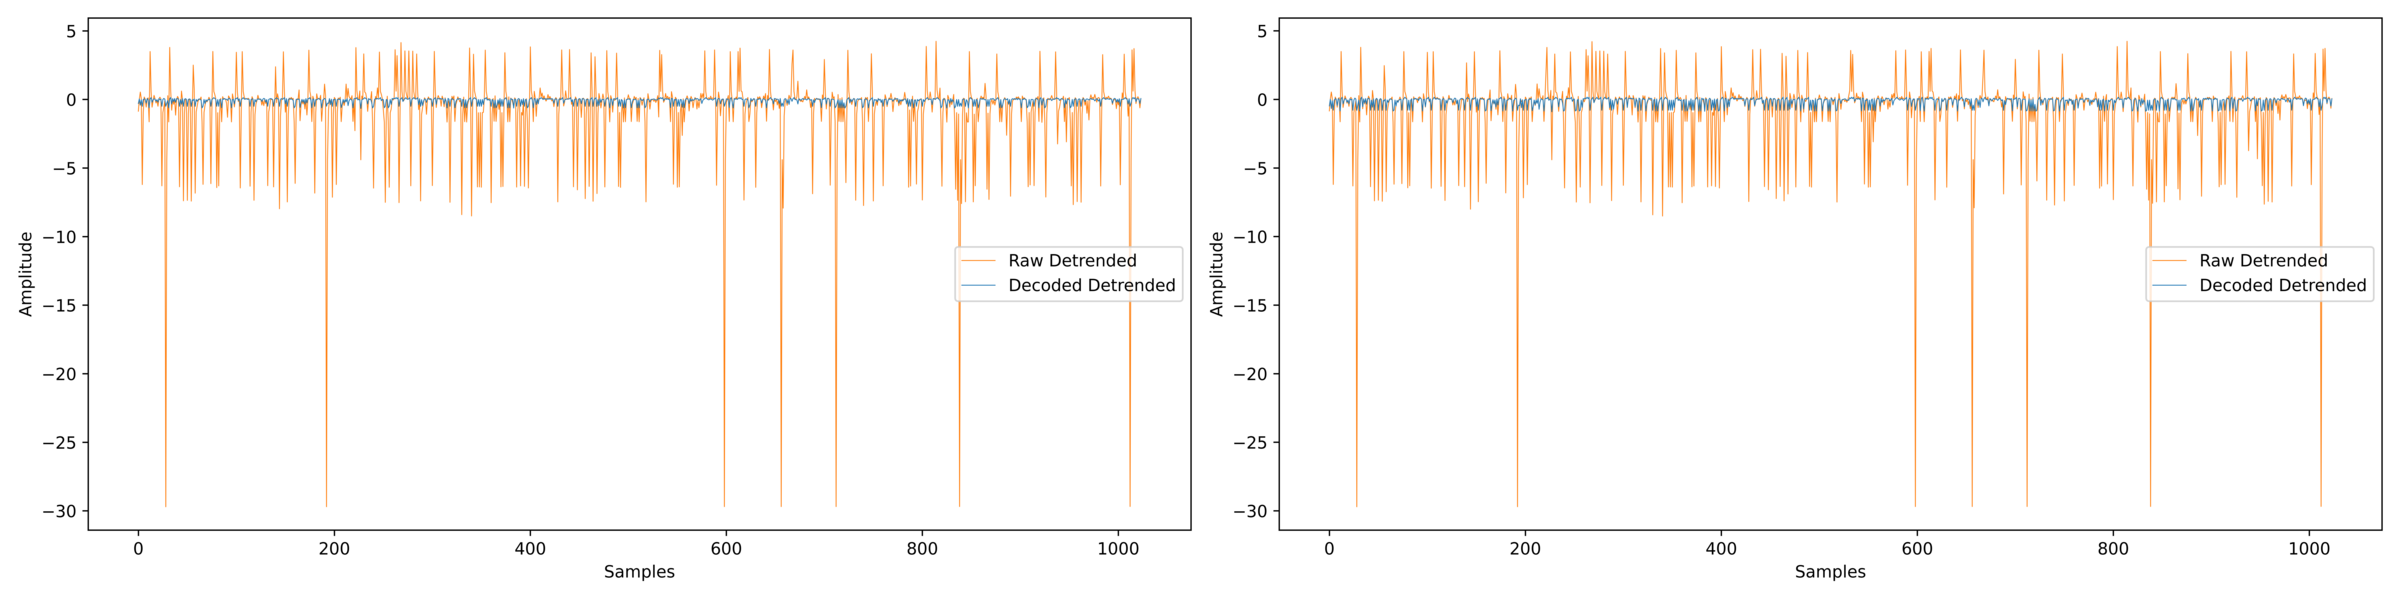
\includegraphics[width=0.8\textwidth]{static/detrended_signal_blend_01_resized.png}
%     \caption{Detrended signals when blend=0.1}
%     \label{fig:detrended_signal_01}
% \end{figure}
% %

% %
% \begin{figure}[ht]
%     \centering
%     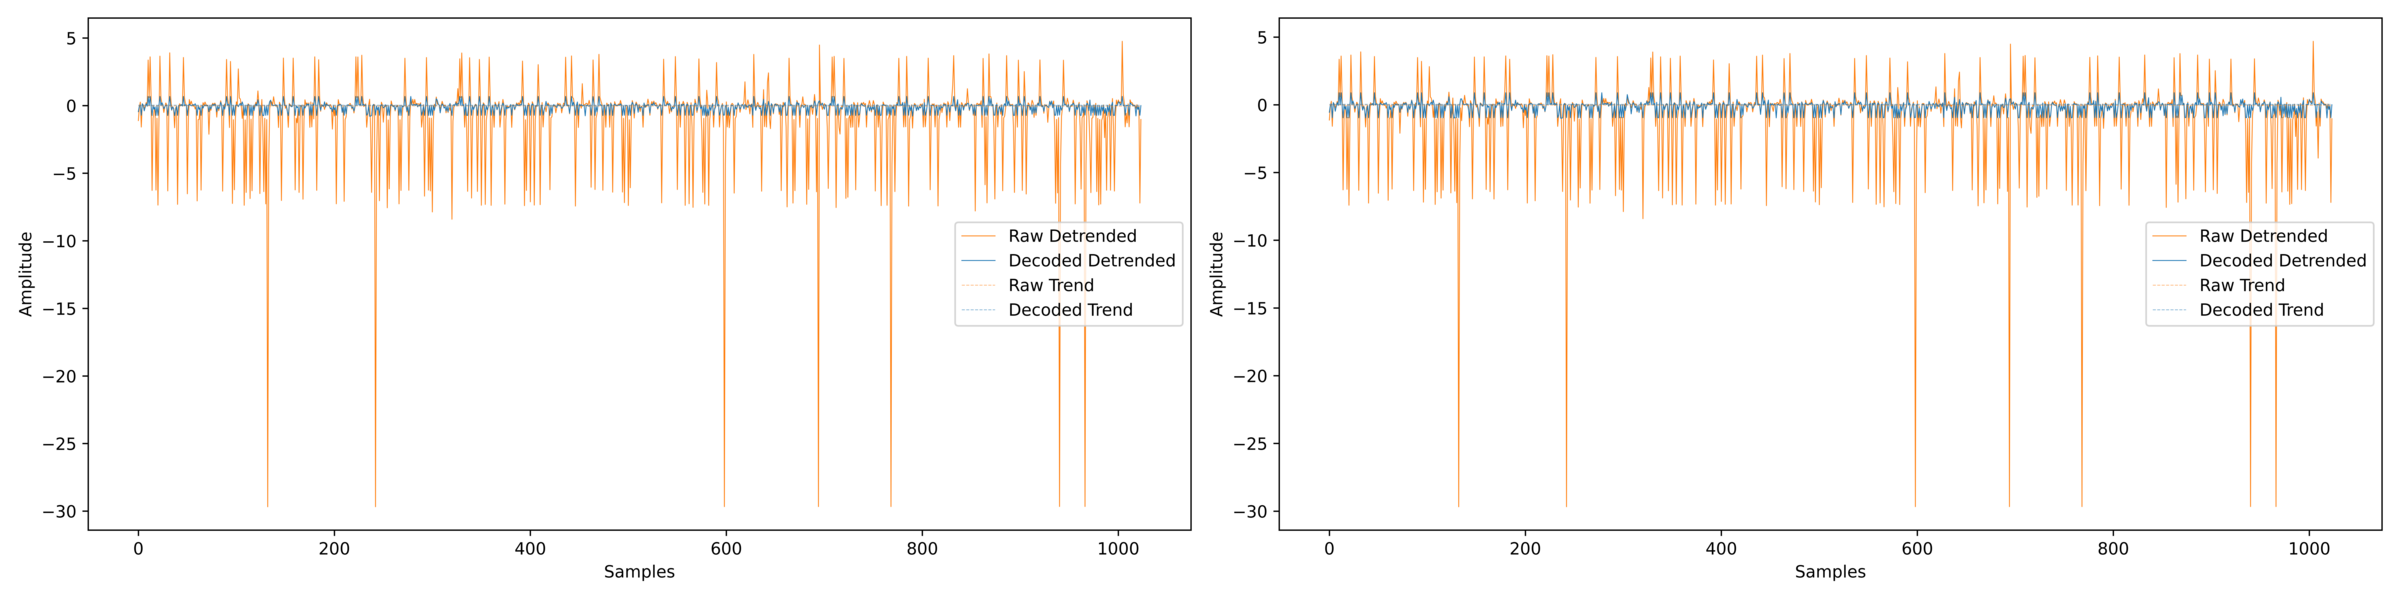
\includegraphics[width=0.8\textwidth]{static/detrended_signal_blend_08_resized.png}
%     \caption{Detrended signals when blend=0.8}
%     \label{fig:detrended_signal_08}
% \end{figure}
% %

% \subsubsection{RMS Analysis} The root mean square (RMS) analysis provides additional insight into the performance of the autoencoder. When the blend is set to 0.1, the majority of the RMS values are centered around zero, with outliers remaining prominent. This result is acceptable but suggests room for improvement. When the blend is set to 0.8, the RMS shows significant improvement, with a higher count of zeros. The outliers continue to exhibit significant values, but overall, the analysis indicates a better reconstruction.
% %
% \begin{figure}[ht]
%     \centering
%     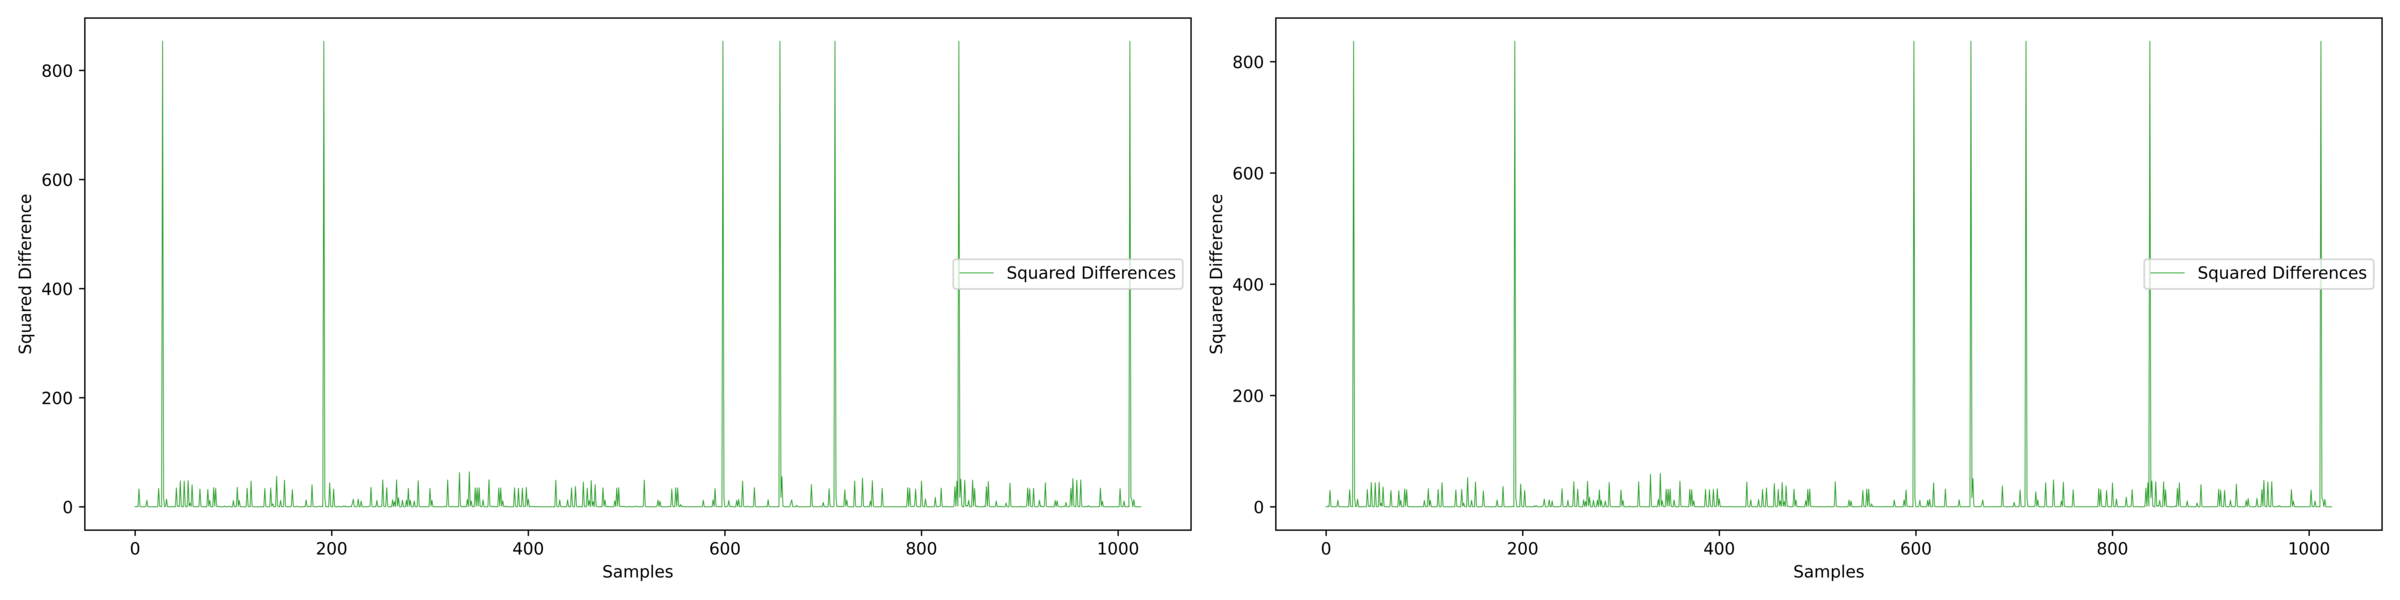
\includegraphics[width=0.8\textwidth]{static/rms_analysis_blend_01_resized.png}
%     \caption{RMS analysis when blend=0.1}
%     \label{fig:rms_analysis_01}
% \end{figure}
% %

% %
% \begin{figure}[ht]
%     \centering
%     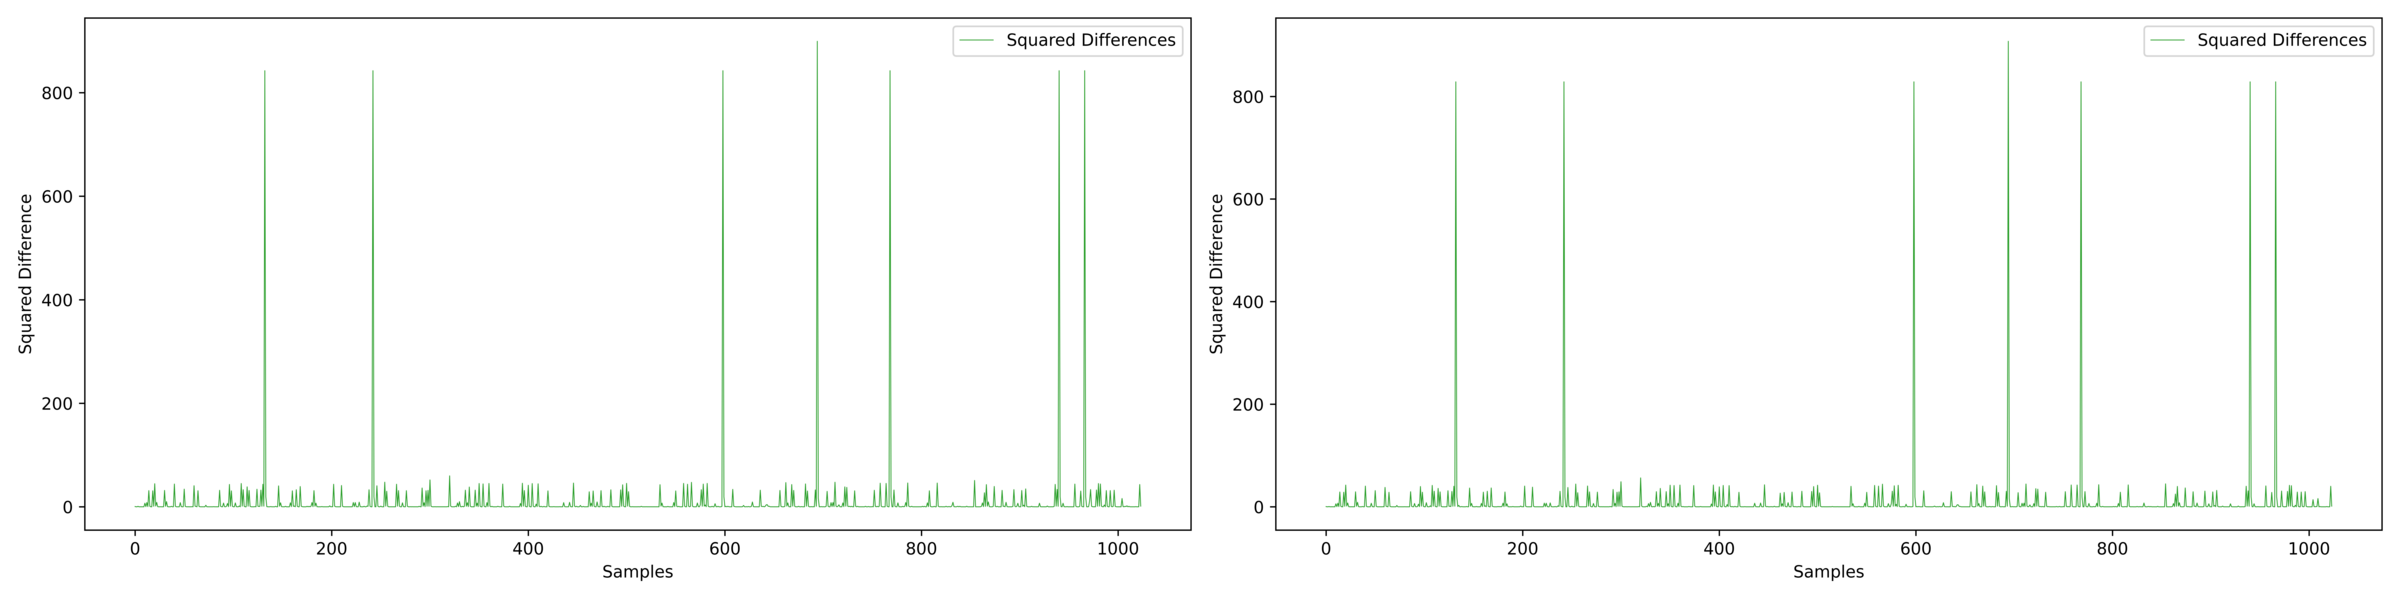
\includegraphics[width=0.8\textwidth]{static/rms_analysis_blend_08_resized.png}
%     \caption{RMS analysis when blend=0.8}
%     \label{fig:rms_analysis_08}
% \end{figure}
% %

% \subsubsection{Band Analysis} When the blend is set to 0.8, the decoded signal exhibits non-zero values across all bands, indicating a more robust amplitude representation. In some bands, the levels of the decoded signal closely match those of the original signal, suggesting that the model effectively captures the corresponding frequency ranges. In contrast, when the blend is set to 0.1, the distributions of the raw and decoded bands differ significantly. Some bands in the decoded signal are nearly zero, while the raw signal contains substantial values, indicating that the amplitude is not well captured.
% %
% \begin{figure}[ht]
%     \centering
%     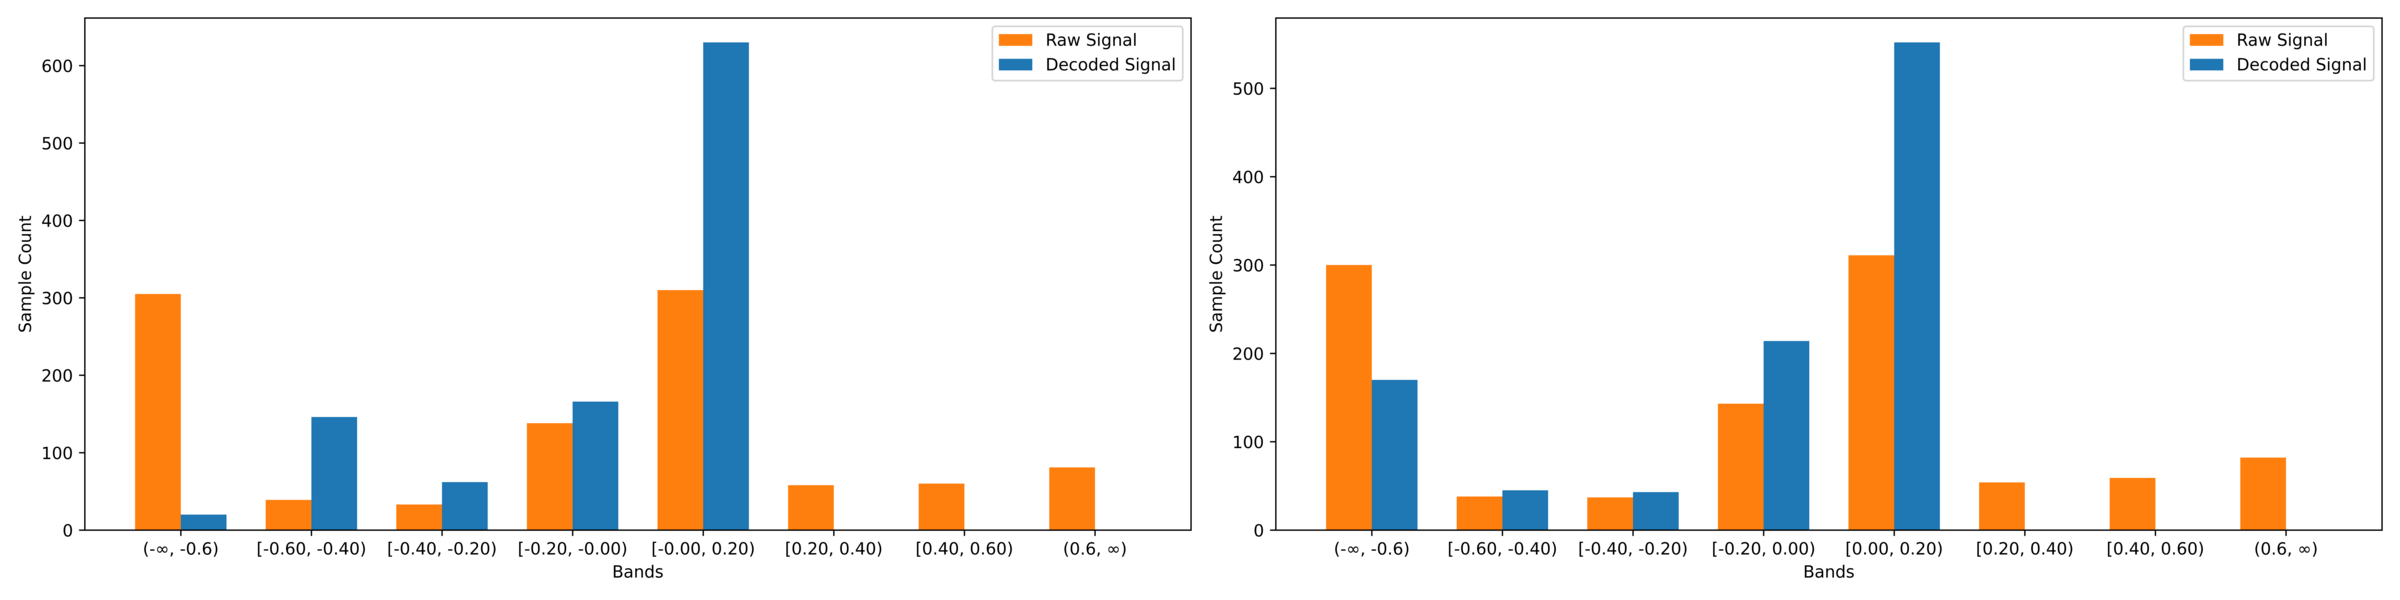
\includegraphics[width=0.8\textwidth]{static/band_analysis_blend_01_resized.png}
%     \caption{Band analysis when blend=0.1}
%     \label{fig:band_analysis_01}
% \end{figure}
% %

% %
% \begin{figure}[ht]
%     \centering
%     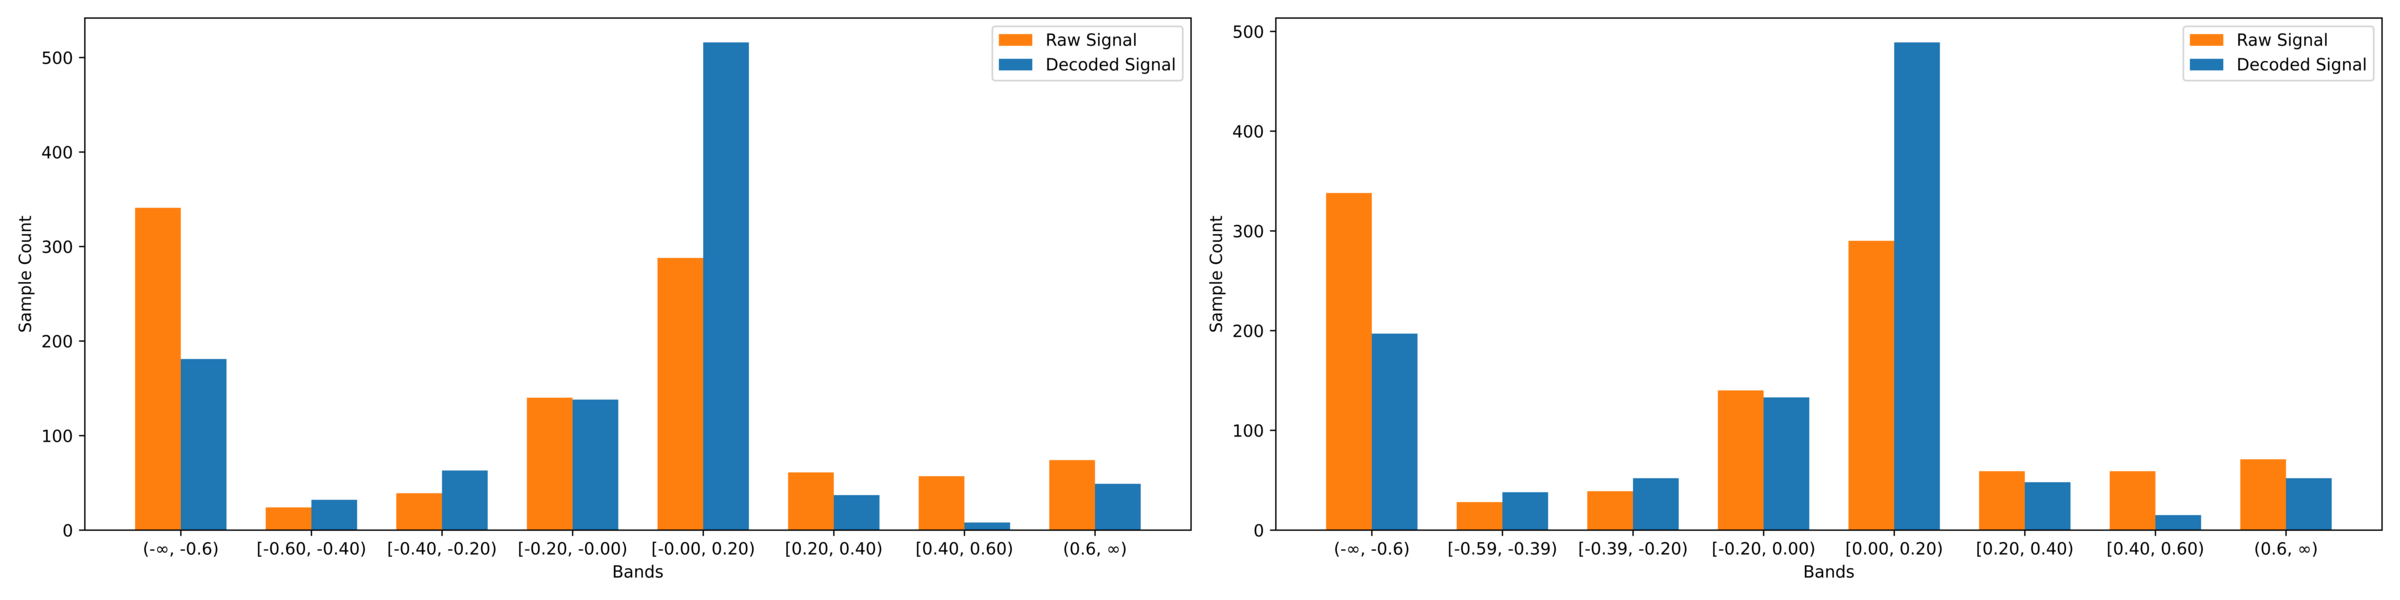
\includegraphics[width=0.8\textwidth]{static/band_analysis_blend_08_resized.png}
%     \caption{Band analysis when blend=0.8}
%     \label{fig:band_analysis_08}
% \end{figure}
% %

% \subsubsection{Other Metrics}

% The performance of the autoencoder is evaluated using various metrics for both blends (0.1 and 0.8). These metrics include band rate differences, zero-crossing rates, RMS values, and Pearson correlation coefficients, calculated as differences between the raw and decoded signals. A smaller difference indicates a closer match to the original signal, which is preferable. Better results are highlighted in blue. Below are the detailed results for each feature and blend setting, showing that the blend with 0.8 is superior.
% %
% \begin{table}[ht]
%     \centering
%     \begin{tabular}{l|c|c}
%         \hline
%         \textbf{Metric} & \textbf{Blend=0.8} & \textbf{Blend=0.1} \\ 
%         \hline
%         Bands \% $F_1$ & 
%         \begin{tabular}[c]{@{}c@{}} 
%         \color{blue}{0.4422} \\ 
%         1.0 \\ 
%         1.0 \\ 
%         -0.1232 \\ 
%         \color{blue}{0.3420} \\ 
%         1.0 \\ 
%         1.0 \\ 
%         \color{blue}{0.3108} 
%         \end{tabular} 
%         & 
%         \begin{tabular}[c]{@{}c@{}} 
%         0.9557 \\ 
%         1.0 \\ 
%         1.0 \\ 
%         \color{blue}{-0.2767} \\ 
%         0.7927 \\ 
%         1.0 \\ 
%         1.0 \\ 
%         1.0 
%         \end{tabular} \\
%         \hline
        
%         Bands \% $F_2$ & 
%         \begin{tabular}[c]{@{}c@{}} 
%         \color{blue}{0.3659} \\ 
%         1.0 \\ 
%         1.0 \\ 
%         \color{blue}{-0.0824} \\ 
%         \color{blue}{0.2217} \\ 
%         1.0 \\ 
%         1.0 \\ 
%         \color{blue}{0.2556} 
%         \end{tabular} 
%         & 
%         \begin{tabular}[c]{@{}c@{}} 
%         0.4524 \\ 
%         1.0 \\ 
%         1.0 \\ 
%         -0.2741 \\ 
%         0.7840 \\ 
%         1.0 \\ 
%         1.0 \\ 
%         1.0 
%         \end{tabular} \\
%         \hline

%         Zero Crossing Rate $F_1$ & 1.3439 & \color{blue}{1.2631} \\ 
 
%         Zero Crossing Rate $F_2$ & 1.3334 & \color{blue}{1.0186} \\ 
 
%         RMS $F_1$ & \color{blue}{2.8682} & 2.9533 \\ 

%         RMS $F_2$ & \color{blue}{2.7980} & 2.8774 \\ 
  
%         Pearson Correlation $F_1$ & \color{blue}{0.6527} & 0.6085 \\ 
   
%         Pearson Correlation $F_2$ & \color{blue}{0.6610} & 0.6364 \\ 
%         \hline
%     \end{tabular}
%     \caption{Comparison of Metrics for Blends 0.1 and 0.8. Metrics are expressed as differences between Raw and Decoded signals.}
%     \label{tab:metrics_comparison}
% \end{table}
% %

\clearpage
\section{Data Distillation}
\label{sec:datdist}
%(M5-M24) (Leader: NUIDUCD-CeADAR, support: NCSR
%"D", FDI, Fraunhofer, INRIA)
\subsection{Introduction}
Considering the efficiency in AI dimension of the MANOLO project, tackling this task from the data perspective will, among other techniques, involve the development Data Distillation methods, which aim to create compact, high-fidelity data summaries from large datasets while retaining essential data patterns and dynamics.

\subsection{Technique One}
Our research into data distillation focused on distilling computer vision datasets, namely MNIST and CIFAR10. The MNIST dataset is a collection of 70,000 grayscale images of handwritten digits (0–9), while the CIFAR-10 dataset consists of 60,000 color images across 10 distinct classes (e.g., animals, vehicles). These datasets are commonly used for training and testing in image classification tasks.
\label{subsec:2.3_datdist_tech1}

\subsubsection{Methodology}

One of the key goals of the MANOLO project is to enable efficient training and deployment of AI models across the Cloud-Edge Continuum (CEC), where computational resources are often constrained. This is where data distillation can align with MANOLO’s efficient AI goals by creating reduced datasets which preserve essential information, thus ensuring faster, lower-memory, and resource-efficient model training. Furthermore, since MANOLO’s techniques are intended for use with diverse data types, data distillation with agnostic techniques (e.g., clustering) will help standardise the data preparation activity across various use cases. 

Our proposed data distillation methodology uses a combination of Variational Autoencoders (VAEs) and K-means clustering to reduce the size of computer vision datasets while maintaining high accuracy metrics when used for classification tasks. Variational Autoencoders are neural networks that encode input data into a compressed latent space, which captures the data's essential features. In our approach, we train a Variational Autoencoder on the dataset in order to generate such a latent space. After this, the latent space is clustered into N clusters, where N is the number of target classes in the dataset being distilled. Since the number of clusters are pre-determined, the clustering algorithm used to achieve this is K-means. Once the clustering process is complete, the centroid of each cluster is calculated and the distances from each latent space encoded sample to its corresponding cluster centroid is found. The measure used to calculate this is Euclidean distance. 

In order to reduce the size of the dataset being distilled, the encoded samples with the shortest distances to their corresponding cluster are found and removed from the dataset. The logic behind this is that these samples are the easiest to classify and contribute the least amount of information to the training process. ...

\subsubsection{Results}


%
\begin{table}[ht]
    \centering
    \begin{tabular}{l|c|c|c|c|c|c|c}
        \hline
        \textbf{Metric} & \textbf{Full Dataset} & \textbf{10\%} & & & & & \\ 
        \hline
        
        Accuracy & 
 0.9
        & 
        0.9  & & & & & \\
        
        Precision & 
        0.9
        & 
        0.9  & & & & & \\

        Recall & 1.3439 & \color{blue}{1.2631}  & & & & & \\ 
 
        F1 Score & 1.3334 & \color{blue}{1.0186}  & & & & &\\ 
 
    \end{tabular}
    \caption{Comparison of Metrics for Blends 0.1 and 0.8. Metrics are expressed as differences between Raw and Decoded signals.}
    \label{tab:dataset_distillation_results}
\end{table}
%



\clearpage
\section{Data and Feature Synthetisation}
\label{sec:datsynth}
\subsection{Introduction}\label{subsec:2.3_intro}
The process of training AI models heavily relies on the quality of the datasets involved, including the quality of the samples, the quality of the annotations, and the amount of samples among other factors. Whilst the MANOLO data quality assessment module, addressed in the previous task in this workpackage, assesses data quality, an overall lack of data during training often leads to bias in model predictions as well as poor model performance at inference time. 

The MANOLO submodule discussed in this section, the Data and Feature Synthetisation submodule, compiles a set of techniques to generate synthetic data in the form of new unseen samples or their equivalent extracted features. This allows the user to address the challenges stemming from a lack of data, whether increasing the overall number of training examples to increase data variability, generating data from a particular class to address class imbalance, or directly mitigating biasses in the dataset. 

The first version of the deliverable reports the efforts undertaken towards data synthetisation through the experimentation with Invertible Neural Networks. These networks are trained on classification datasets, then, they can generate a new sample compatible with a given label, according to the learned parameters of the network. Section~\ref{subsec:2.3_datasynth_tech1} introduces the technique as it will be part of the MANOLO library, in the conditional version (cINNs). The initial cINNs implementation for the MANOLO data module allows the generation of samples from a dataset and the generative condition extends from a particular class to a style contained in the latent space.

    %%%%%%%%%%%%%%%% Conditional Invertible Neural Networks  %%%%%%%%%%%%%%%%
    \subsection{Conditional INNs}
    \label{subsec:2.3_datasynth_tech1}

        In this subsection we address data generation with the conditional invertible neural networks proposed by Ardizonne et al.~\cite{2019_arxiv_cinn}. Conditional Invertible Neural Networks (cINNs) are a variation of invertible neural networks that provide an efficient solution to conditional data generation. INNs need to be, by definition, bijective, which constrains their possible architectures, as batch normalization and pooling layers are not invertible. When conditional generation is introduced, these INNs are combined with an unconstrained NN for that task. The conditional neural network can be used as a processing unit too, which implies operations similar as those not invertible. INNs behave as a transport map between the input distribution and the latent distribution. In the case of computer vision, for instance, INNs map an image $\mathbf{x}$ from the image space (RGB representation) to one latent vector $\mathbf{z}$, without the need of a posterior, as is the case for Variational Autoencoders. This deliverable will show an initial exploration of class and style conditioning alternatives. These approaches allow the model to generate class conditioned images with a particular style living in the latent space.
        
        \subsubsection{Methodology}

            This subsection describes the technical aspects of the approach selected as a basic introduction to background concepts underlying the INN implementation, the approach proposed in~\cite{2019_arxiv_cinn} to condition the sample generation with class labels, the adaptation we proposed to condition the style of the generated samples, and a description of the experimental setup used to obtain the results reported in the following subsection.
         
            \paragraph{Class-conditioned sample generation.} 
            Sample generation with INNs, as with normalising flows [GLOW NeurIPS2018 - Kingma and Dhariwail], is based on the principle behind the change of variable statistics formula $p_{X}(X) = p_{Z}(f(X))|\det Df(X)|^{-1}$, where $p_{X}(X)$ and $p_{Z}(f(X))$ are the probability distributions from the input and the latent space respectively, $\det Df(X)$ is the determinant of the Jacobian of $f(X)$, and $f(X)$ is the model or mapping function that we are going to learn. We train this model, as is most commonly done, via maximum likelihood. Following the mathematical developments by Ardizonne et al.~\cite{2019_arxiv_cinn}, which include the prior conditioning of the model, this results in the minimization of three terms: the squared module of the model prediction, the logarithm of the Jacobian of the model weights, and a regularization to enforce a Gaussian space being learned. 
                        
            Class-conditioned sample generation relies on a prior introduced during training and inference to alter the mapping and constrict it to a particular region of the latent space, a region that belongs to the samples under the given condition. The prior used in our experiments consist of a one-hot-encoded vector, representing the semantic class of a sample, concatenated to the internal representations of the blocks that compose the INN. This is shown in Figure~\ref{fig:class_cond_gen},  where the input $z_i$ is a random Gaussian noise vector, the condition $c_i$ is a vector indicating the class ``3'' in this particular example, and the output $x_i$ is a newly generated image of a digit ``3''. By using different noise vectors as seeds for the generation of the samples, the model outputs different new samples all corresponding to the category indicated by the condition vector. 

            \begin{figure}
                \vskip -0.2in 
                \centering
    
                \includegraphics[width=0.80\columnwidth]{Images/schema_con_gen.png} 
                
                \vspace{-2pt}
                \caption{\label{fig:class_cond_gen} Schematic.... class conditional image generation.}
                \vskip -0.0in 
            \end{figure}
        
            \paragraph{Style-and-class-conditioned sample generation.} 
            Style-and-class-conditioned sample generation goes a step farther, assumes that the class condition is fixed, and conditions the sample generation to adhere to a particular style. We define the style by exploring the latent space learned by the INN and select a set of seed noise vectors near an area of interest, i.e. the noise vectors corresponding to a set of samples that exhibit the style we are interested in. Since different latent vectors result in different images being generated, by moving a random noise vector towards a region in the latent space where a particular set of samples belong, we condition the generation of samples. This is depicted Figure~\ref{fig:ciinn_latent_conditioning}. 
            
            To define the region of the latent space that contains the style we want, we define a style vector $z_s$ that represents the style we are interested in. We do this by manually selecting $K$ samples that share the particular style we want (bold, italic, faint writing styles in the MNIST example) and mapping them to the latent space, resulting in a latent style vector per sample $\{z_{s1}, z_{s2}, ..., z_{sK}\}$. Then we define the style vector as the centroid of the individual style vectors $z_{s} = 1/K \sum_{i} z_{si}$. Finally, we generate samples using the interpolation of $z_{s}$ with a random Gaussian noise vector $z_i$ as a conditioned seed vector $z_c = (1-t) z_i + t z_{s}$ that falls close to a region in the latent space that encodes a particular style (boldness in the example in Figure~\ref{fig:ciinn_latent_conditioning}). The strength of that interpolation modulates how close the $z_c$ vector is to the style vector $z_s$ and, consequently, how strong will the presence of the particular style be in the generated image.
            
            \begin{figure}
                \vskip -0.2in 
                \centering
    
                \includegraphics[width=0.90\columnwidth]{Images/schematic_latent_space_cond_cinn.png} 
                
                \vspace{-2pt}
                \caption{\label{fig:ciinn_latent_conditioning} Schematic.... conditioning the latent space with z\_i seeds}
                \vskip -0.0in 
            \end{figure}
    
            \paragraph{Experimental setup.} 
            The sample generation functionality for the Data Inspection and Genration MANOLO submodule is currently developed and tested on the MNIST dataset~\cite{1998_IEEE_MNIST}. This is a small dataset, widely used in the research community that allows for faster and simpler exploration. MNIST contains 60000 black and white 28$\times$28 images of hand written digits group into ten different classes corresponding to the digits from zero to nine. The experiments presented in this section use the INN model  proposed in~\cite{2019_arxiv_cinn}, composed of 20 linear layers as implemented in the FrEIA library~\cite{freia}. Hence, the images are flattened into a 784 dimensional vector in the input of the model and then unflattened back at the output. The INN is trained on 256 samples batches with Adam optimizer and an learning rate of $1e-5$ that we reduced by a factor of 10 at epoch 20 and epoch 40 of a 60 epochs training. We are currently exploring the implementation of larger models including convolutional layers and aim to include this or alternative models that scale to larger datasets in a future report. Please refer to the future work section (link to the right section) for more details.

        \subsubsection{Results}
            \paragraph{Class-conditioned sample generation.} 
            The experiments on class-conditional sample generation illustrate the ability of a cINN to generate samples from a given class. The network is trained to map samples from the image space $p_X$ to the latent space $p_Z$ conditioned to a particular class. Then, the learned model, when inverted, is able to map a randomly generated seed vector $z_i$, a Gaussian noise vector, to a new sample $x_i$ never seen by the model. To illustrate this, Figure~\ref{fig:exp_class_cond} shows several examples of images generated with a trained cINN. In particular, each column shows samples generated from a single seed vector and different conditions for the class that range from from 0 to 9. On the other hand, each row shows samples generated with a fixed class condition and different input seed vectors $z_i$.

            \begin{figure}
                \vskip -0.2in 
                \centering
    
                \includegraphics[width=0.20\columnwidth]{Images/empty_image.png} 
                
                \vspace{-2pt}
                \caption{\label{fig:exp_class_cond} Schematic.... }
                \vskip -0.0in 
            \end{figure}

            \paragraph{Style-and-class-conditioned generation.} 
            The results from the class-conditional sample generation experiments use different seeds to generate different samples under the same class condition. Then, the results in this section demonstrate how we further condition the sample generation process to enforce a particular style to the newly generated samples. Figures~\ref{fig:exp_stle_1}, \ref{fig:exp_stle_3}, and~\ref{fig:exp_stle_1}, provide examples of style-and-class conditioned generated samples and the corresponding initial seeds. These figures help illustrate the generation process: the left-most column contains 10 samples manually selected that belong to a particular style, bold, italic, and xxxx respectively; then the following 10 columns correspond to the samples generated for the ten different class conditions (digits from zero to nine), and each row from top to bottom, correspond to an increasing level of style conditioning strength. The top row samples are generated from a completely random seed vector, the bottom row samples from the style vector $z_s$ obtained from the manually selected samples, and the rows in between interpolations of these vectors. The strength of the interpolation , and of the conditioning consequently, is defined by the parameter $t$ and in these results is linearly increased between zero and one. 

            \begin{figure}
                \vskip -0.2in 
                \centering
    
                \includegraphics[width=0.20\columnwidth]{Images/empty_image.png} 
                
                \vspace{-2pt}
                \caption{\label{fig:exp_stle_1} Schematic.... }
                \vskip -0.0in 
            \end{figure}

            \begin{figure}
                \vskip -0.2in 
                \centering
    
                \includegraphics[width=0.20\columnwidth]{Images/empty_image.png} 
                
                \vspace{-2pt}
                \caption{\label{fig:exp_stle_2} Schematic.... }
                \vskip -0.0in 
            \end{figure}

            \begin{figure}
                \vskip -0.2in 
                \centering
    
                \includegraphics[width=0.20\columnwidth]{Images/empty_image.png} 
                
                \vspace{-2pt}
                \caption{\label{fig:exp_stle_3} Schematic.... }
                \vskip -0.0in 
            \end{figure}

        
            %%%%%%%%%%%%%%%%%%%%%%%%%%%%%%%%%%%%%%%%%%%%%%%%%%%%%%
            %%%%%% not reviewed.... still work to be done here 
            \paragraph{Still to unfinished:}
                \begin{enumerate}
                    \item Preliminary tests with FashionMNIST - still to try out
                    \item Conv-cINN? - so far they do not train well...
                    \item can we move to CIFAR? - we would need to have the convINN running for this
                \end{enumerate}
            %%%%%%%%%%%%%%%%%%%%%%%%%%%%%%%%%%%%%%%%%%%%%%%%%%%%%%


\clearpage
\section{Feature Extraction}
\label{sec:featextr}

Feature extraction intro

\subsection{Technique One}
\label{subsubsec:2.3_featext_tech1}

\subsubsection{Methodology}

\subsubsection{Results}	


\clearpage
\section{Conclusion}

\bibliographystyle{plain}
\bibliography{refs}

\end{document}
